%%%%%%%%%%%%%%%%%%%%%%%%%%%%%%%%%%%%%%%%%
% Short Sectioned Assignment LaTeX Template Version 1.0 (5/5/12)
% This template has been downloaded from: http://www.LaTeXTemplates.com
% Original author:  Frits Wenneker (http://www.howtotex.com)
% License: CC BY-NC-SA 3.0 (http://creativecommons.org/licenses/by-nc-sa/3.0/)
%%%%%%%%%%%%%%%%%%%%%%%%%%%%%%%%%%%%%%%%%

%----------------------------------------------------------------------------------------
%	PACKAGES AND OTHER DOCUMENT CONFIGURATIONS
%----------------------------------------------------------------------------------------

\documentclass[paper=a4, fontsize=11pt]{scrartcl} % A4 paper and 11pt font size

% ---- Entrada y salida de texto -----

\usepackage[T1]{fontenc} % Use 8-bit encoding that has 256 glyphs
\usepackage[utf8]{inputenc}
%\usepackage{fourier} % Use the Adobe Utopia font for the document - comment this line to return to the LaTeX default

% ---- Idioma --------

\usepackage[spanish, es-tabla]{babel} % Selecciona el español para palabras introducidas automáticamente, p.ej. "septiembre" en la fecha y especifica que se use la palabra Tabla en vez de Cuadro

% ---- Otros paquetes ----

\usepackage{amsmath,amsfonts,amsthm} % Math packages
%\usepackage{graphics,graphicx, floatrow} %para incluir imágenes y notas en las imágenes
\usepackage{graphics,graphicx, float} %para incluir imágenes y colocarlas

% Para hacer tablas comlejas
%\usepackage{multirow}
%\usepackage{threeparttable}

%\usepackage{sectsty} % Allows customizing section commands
%\allsectionsfont{\centering \normalfont\scshape} % Make all sections centered, the default font and small caps

\usepackage{fancyhdr} % Custom headers and footers
\pagestyle{fancyplain} % Makes all pages in the document conform to the custom headers and footers
\fancyhead{} % No page header - if you want one, create it in the same way as the footers below
\fancyfoot[L]{} % Empty left footer
\fancyfoot[C]{} % Empty center footer
\fancyfoot[R]{\thepage} % Page numbering for right footer
\renewcommand{\headrulewidth}{0pt} % Remove header underlines
\renewcommand{\footrulewidth}{0pt} % Remove footer underlines
\setlength{\headheight}{13.6pt} % Customize the height of the header

\numberwithin{equation}{section} % Number equations within sections (i.e. 1.1, 1.2, 2.1, 2.2 instead of 1, 2, 3, 4)
\numberwithin{figure}{section} % Number figures within sections (i.e. 1.1, 1.2, 2.1, 2.2 instead of 1, 2, 3, 4)
\numberwithin{table}{section} % Number tables within sections (i.e. 1.1, 1.2, 2.1, 2.2 instead of 1, 2, 3, 4)

\setlength\parindent{0pt} % Removes all indentation from paragraphs - comment this line for an assignment with lots of text

\newcommand{\horrule}[1]{\rule{\linewidth}{#1}} % Create horizontal rule command with 1 argument of height

% paquetes para mostrar el código mas bonito... http://stackoverflow.com/questions/586572/make-code-in-latex-look-nice
\usepackage{color}
\usepackage{listings}
\lstset{ %
language=C++,                % choose the language of the code
basicstyle=\footnotesize,       % the size of the fonts that are used for the code
numbers=left,                   % where to put the line-numbers
numberstyle=\footnotesize,      % the size of the fonts that are used for the line-numbers
stepnumber=1,                   % the step between two line-numbers. If it is 1 each line will be numbered
numbersep=5pt,                  % how far the line-numbers are from the code
backgroundcolor=\color{white},  % choose the background color. You must add \usepackage{color}
showspaces=false,               % show spaces adding particular underscores
showstringspaces=false,         % underline spaces within strings
showtabs=false,                 % show tabs within strings adding particular underscores
frame=single,           % adds a frame around the code
tabsize=2,          % sets default tabsize to 2 spaces
captionpos=b,           % sets the caption-position to bottom
breaklines=true,        % sets automatic line breaking
breakatwhitespace=false,    % sets if automatic breaks should only happen at whitespace
escapeinside={\%*}{*)}          % if you want to add a comment within your code
}


%----------------------------------------------------------------------------------------
%	TÍTULO Y DATOS DEL ALUMNO
%----------------------------------------------------------------------------------------

\title{	
\normalfont \normalsize 
\textsc{{\bf Ingeniería de Servidores (2014-2015)} \\ Grado en Ingeniería Informática \\ Universidad de Granada} \\ [25pt] % Your university, school and/or department name(s)
\horrule{0.5pt} \\[0.4cm] % Thin top horizontal rule
\huge Memoria Práctica 4 \\ % The assignment title
\horrule{2pt} \\[0.5cm] % Thick bottom horizontal rule
}

\author{Jose Arcos Aneas} % Nombre y apellidos

\date{\normalsize\today} % Incluye la fecha actual

%----------------------------------------------------------------------------------------
% DOCUMENTO
%----------------------------------------------------------------------------------------

\begin{document}

\maketitle % Muestra el Título

\newpage %inserta un salto de página

\tableofcontents % para generar el índice de contenidos

\listoffigures


\newpage



%----------------------------------------------------------------------------------------
%	Cuesti´on 1
%----------------------------------------------------------------------------------------

\section{Instale la  aplicación. ¿Qué comando permite listar los benchmarks disponibles?}

En ubuntu, podemos instalarlo simplemente usando (como root) el comando:
\textit{apt-get install phoronix-test-suite.}

Una vez instalado, tenemos que ejecutarlo, para que nos pregunte sí queremos aceptar la licencia y sí queremos permitir enviar a los desarrolladores estadísticas anónimas para mejorar el programa. Para ello escribimos:
\textit{ phoronix-test-suite}
Para listar los benchmarks disponibles, podemos utilizar los siguiente comando:
\textit{phoronix-test-suite list-available-tests} - Para listar los benchmarks
\textit{phoronix-test-suite list-available-suites} - Para listar las suites
Para listar los benchmark que tenemos hemos de utilizer el commando: 
\textbf{phoronix-test-suite list-tests}

\begin{figure}[H]
\begin{center}
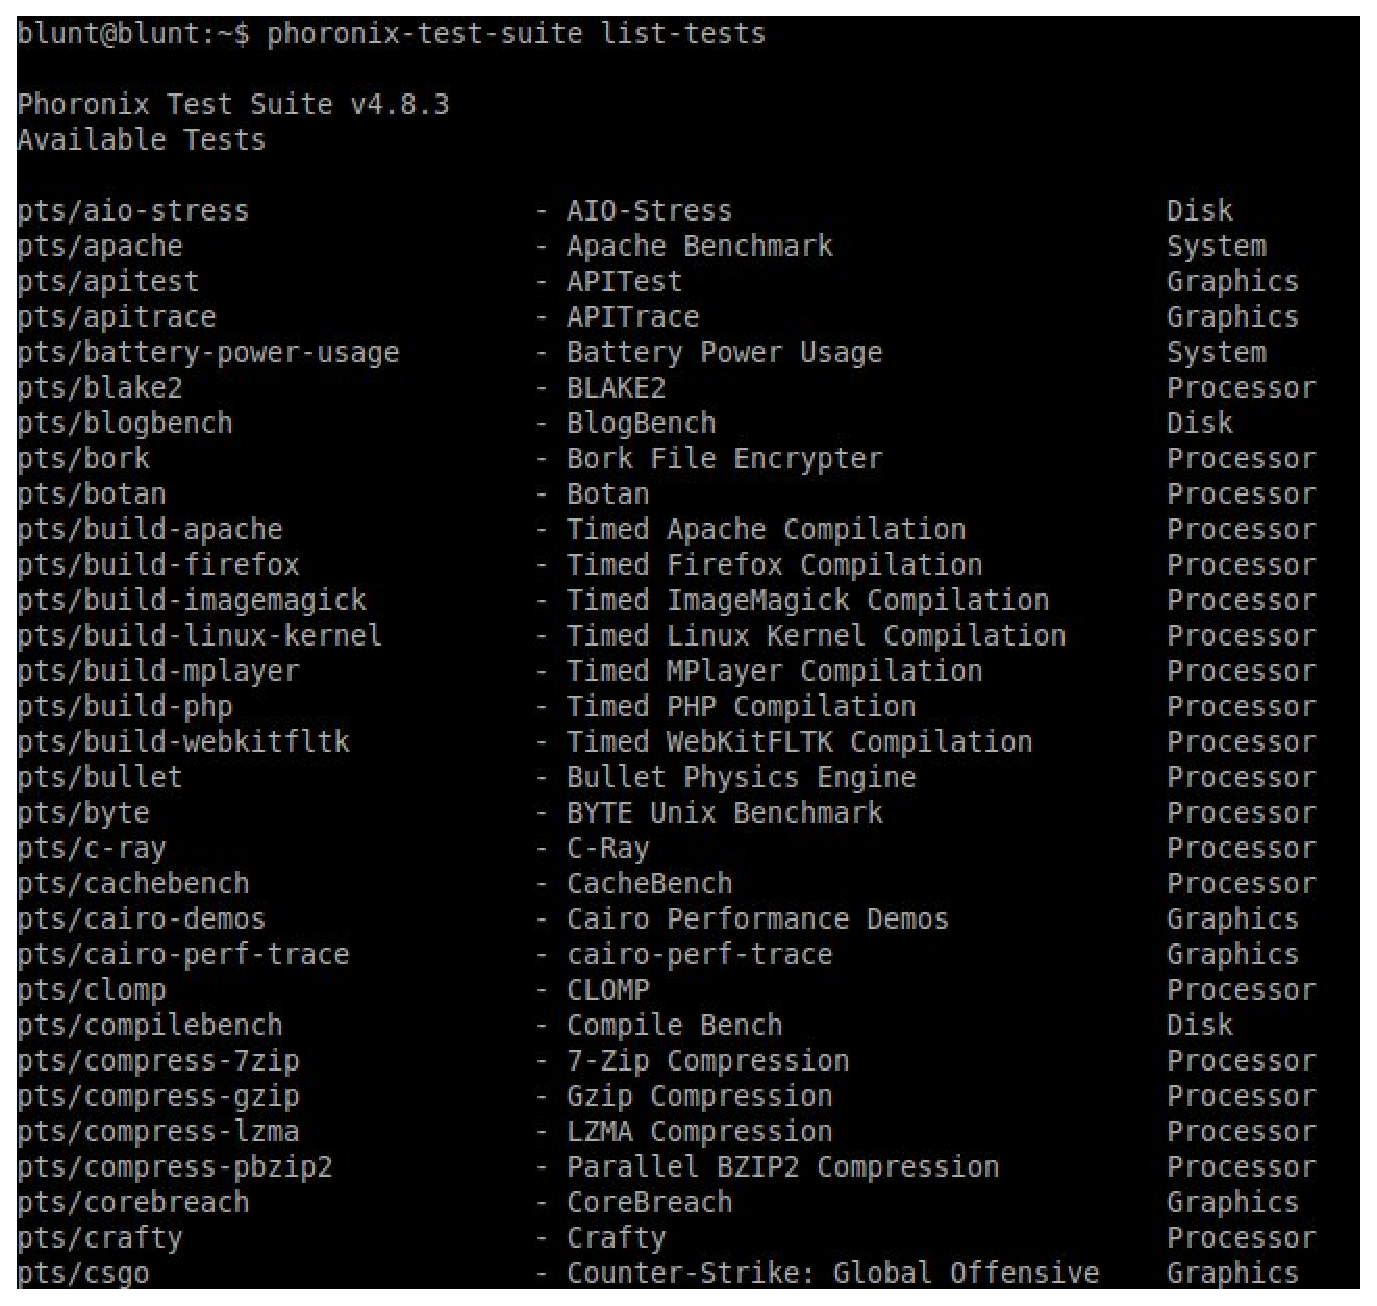
\includegraphics[scale=0.4]{imagenes/imagen1.eps}
\caption{Listado de bechmarks disponibles con phoronix-test-suite list-tests.}
\end{center}
\end{figure}
\footnote{http://www.phoronix-test-suite.com/}
\section{De los parámetros que le podemos pasar al comando ¿Qué significa -c 30 ? ¿y -n 1000?}
La opción -c concurrencia indica el número máximo de peticiones que se podrán
ejecutar simultáneamente. Con -c 30 lo ponemos a 30.
La opción -n peticiones establece el número de peticiones de página web que se
harán al servidor. Con -n 1000 establecemos que se hagan mil peticiones.

\footnote{http://httpd.apache.org/docs/2.2/programs/ab.html}


\section{Ejecute ab contra a las tres máquinas virtuales (desde el SO anfitrión a las máquina virtuales de la red local) una a una (arrancadas por separado) y muestre las estadísticas. ¿Cuál es la que proporciona mejores resultados? Fíjese en el número de bytes transferidos, ¿es igual para cada máquina?}
En primer lugar  \textit{ab} se instala con el comando \textbf{apt-get install apache2-utils}. Una vez instalado podemos generar un benchmarking de la pagina de que deseemos.
En lugar de copiar y pegar el resultado de cada una de las salidas de este comando en cada uno de los servidores se han generado tres graficas en relacion al numero de peticiones y el tiempo que se ha consumido para su realizacion.
El ejercicio pide que nos que comprobemos si se han transferido el numero cuya respuesta es que no. Cada servidor transfiere un número distinto de bytes.

\textbf{Windows}
\begin{figure}[H]
\begin{center}
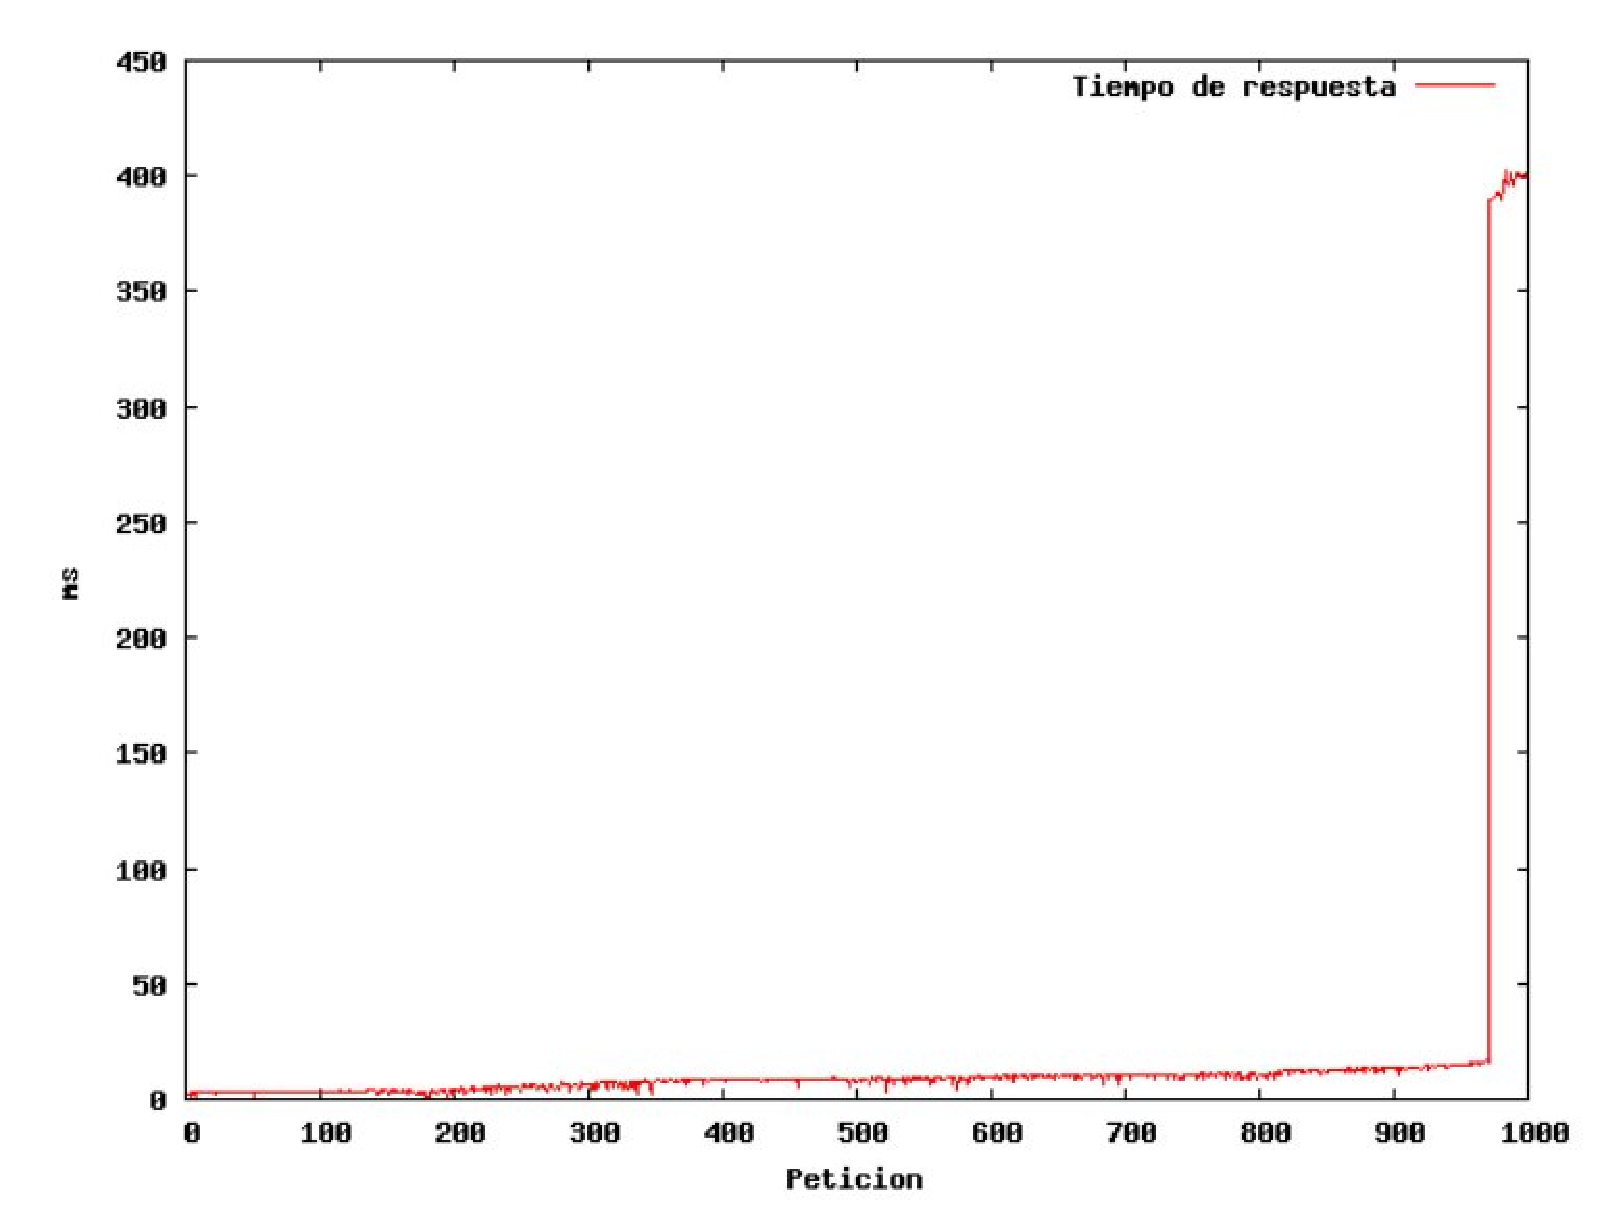
\includegraphics[scale=0.3]{imagenes/imagen3-1.eps}
\caption{Grafica de Windows.}
\end{center}
\end{figure}
\textbf{CentOs} 
\begin{figure}[H]
\begin{center}
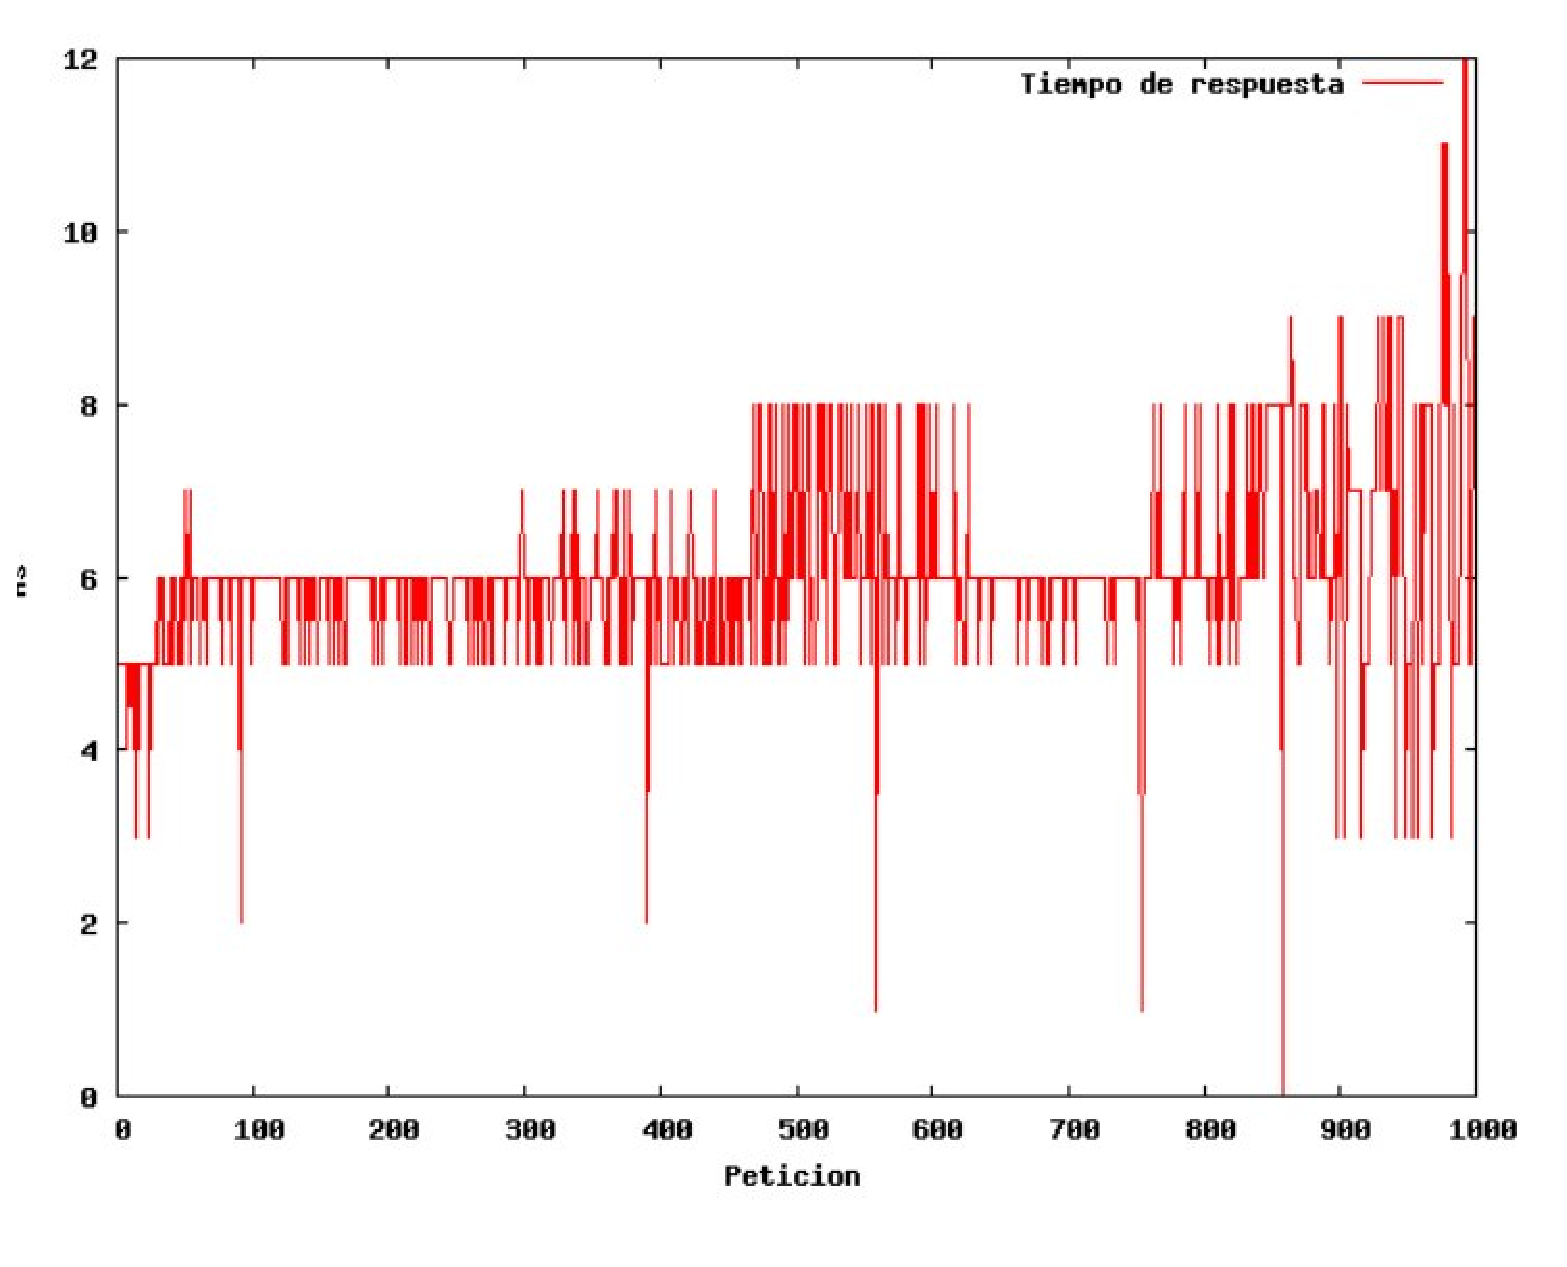
\includegraphics[scale=0.3]{imagenes/imagen3-2.eps}
\caption{Grafica de CentOS.}
\end{center}
\end{figure}
\textbf{Ubuntu}
\begin{figure}[H]
\begin{center}
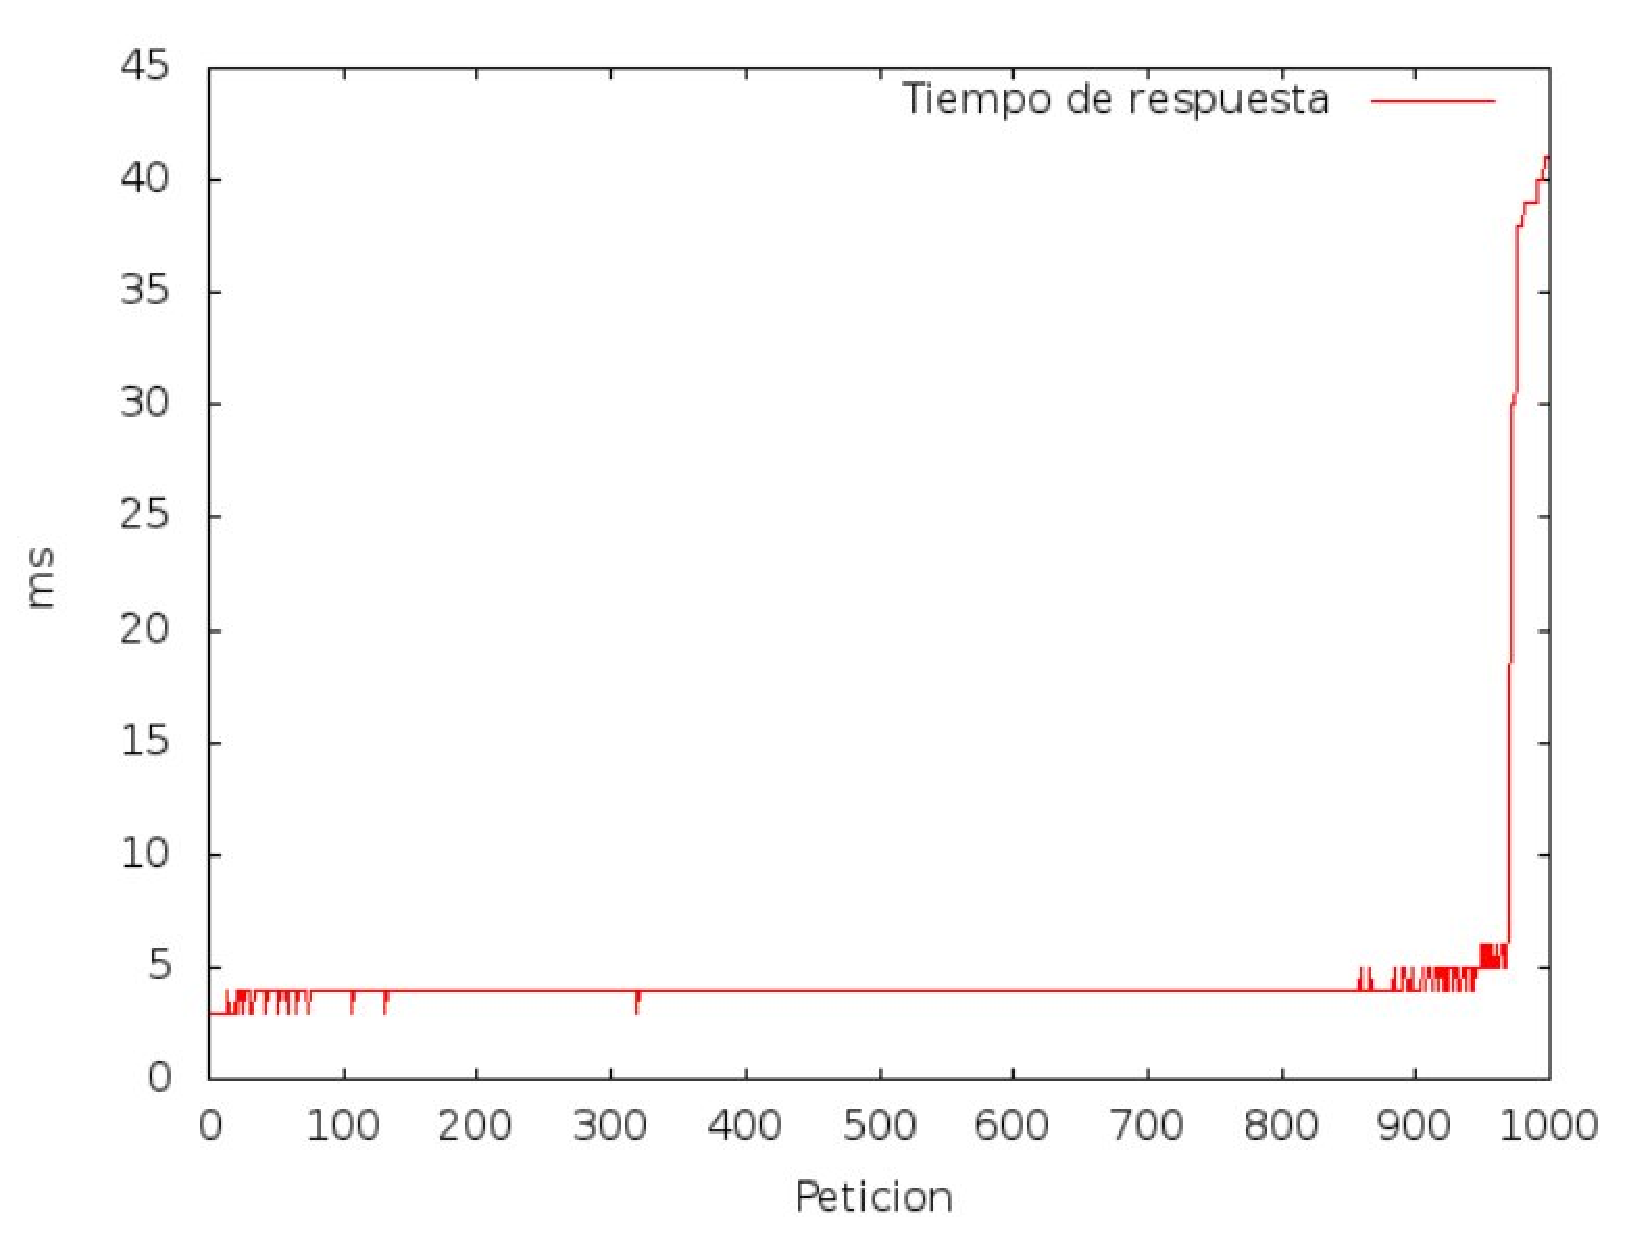
\includegraphics[scale=0.3]{imagenes/imagen3-3.eps}
\caption{Grafica de Ubuntu.}
\end{center}
\end{figure}

Se ha realizado 3 gráficas una por cada servidor, con su tiempo de  respuesta. Con el comando \textit{“ab –c 30 –n 1000 http://<servidor>” }

Puede observarse que se han puesto las gráficas en orden, de mayor tiempo a menor tiempo. Se puede ver como el que peor tiempo de respuesta es el de Windows server. (Aunque no se distinga 
exactamente los valores que toma) Al final ser sobrecarga demasiado y tarda hasta 40-50 veces más de lo normal. Y después le sigue, con un tiempo un poco más constante la máquina CentOs que aunque también se le envíen 1000 peticiones no llega a sobrecargarse tanto como la de Windows. Pero de media tiene unos tiempo un poco peores que los de Ubuntu. 
Y finalmente Ubuntu Server tiene unos tiempo constantes inferiores a 5 ms, pero llega un momento en el que se sobrecarga y comienza a tardar hasta 20 veces más lento. 

\section{Instale y siga el tutorial en http://jmeter.apache.org/usermanual/build-web-test-plan.html realizando capturas de pantalla y comentándolas. En vez de usar la web de jmeter, haga el experimento usando alguna de sus máquinas virtuales (Puede hacer una página sencilla, usar las páginas de phpmyadmin, instalar un CMS, ATC.).}

Después de instalarlo, con los comando de siempre (apt-get install jmeter), lo ejecutamos, hacemos click derecho en “Plan de Pruebas” y seleccionamos Añadir - Grupo de Hilos. Lo modificamos y lo dejamos con estos parametros:

\begin{figure}[H]
\begin{center}
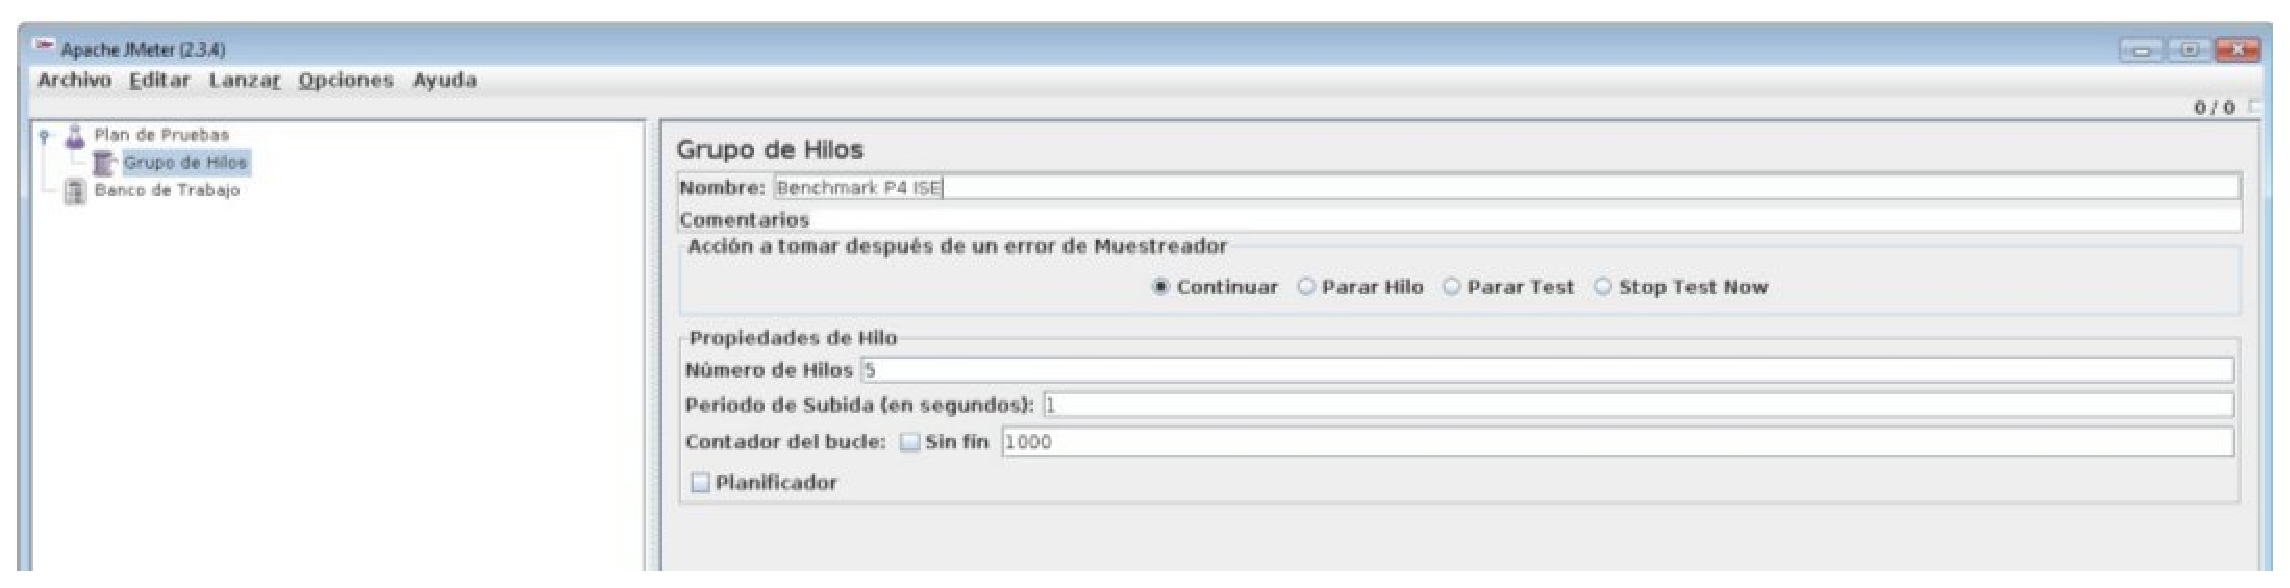
\includegraphics[scale=0.4]{imagenes/imagen4-1.eps}
\caption{Seleccion del grupo de hilos.}
\end{center}
\end{figure}

Ahora creamos las opciones por defecto para las consultas HTTP. Para ello, click  derecho, Añadir - Elementos de Configuración - Valores por defecto para  Petición HTTP. Lo dejamos con estas opciones:
\begin{figure}[H]
\begin{center}
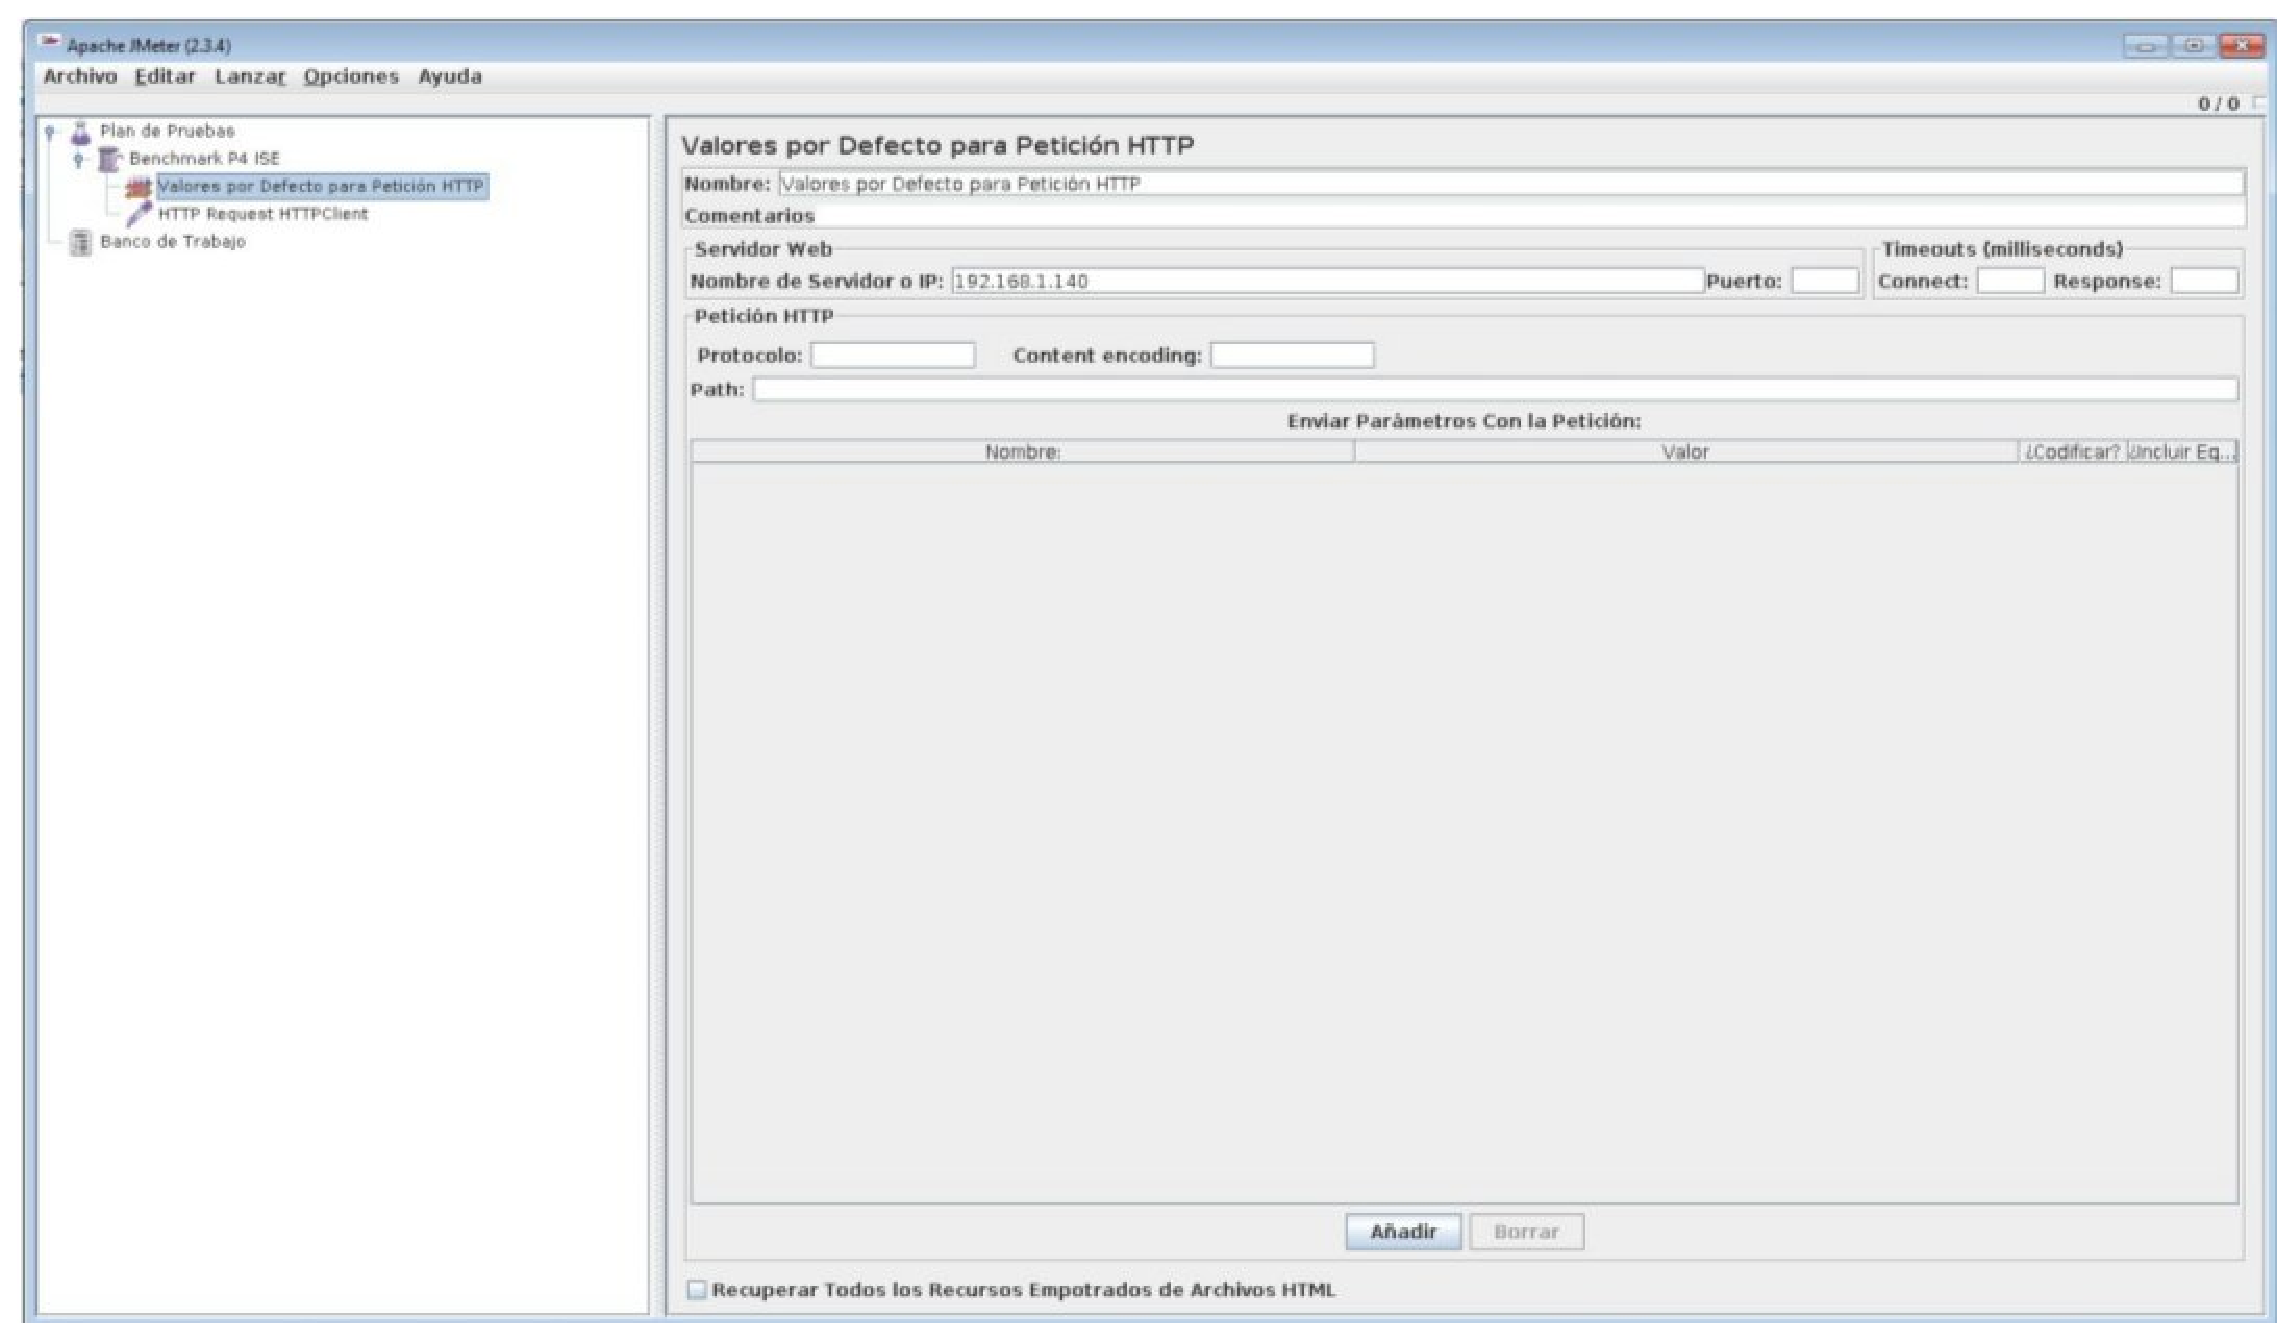
\includegraphics[scale=0.3]{imagenes/imagen4-2.eps}
\caption{Creacion de opciones para consulta HTTP.}
\end{center}
\end{figure}

Después creamos dos consultas HTTP. Una nos llevará al directorio raíz, otra a una  página con imágenes. Para añadir las consultas sería pulsar Añadir -- Muestreador -- HTTP Request HTTP client. Añadimos dos y dejamos estos parámetros:

\begin{figure}[H]
\begin{center}
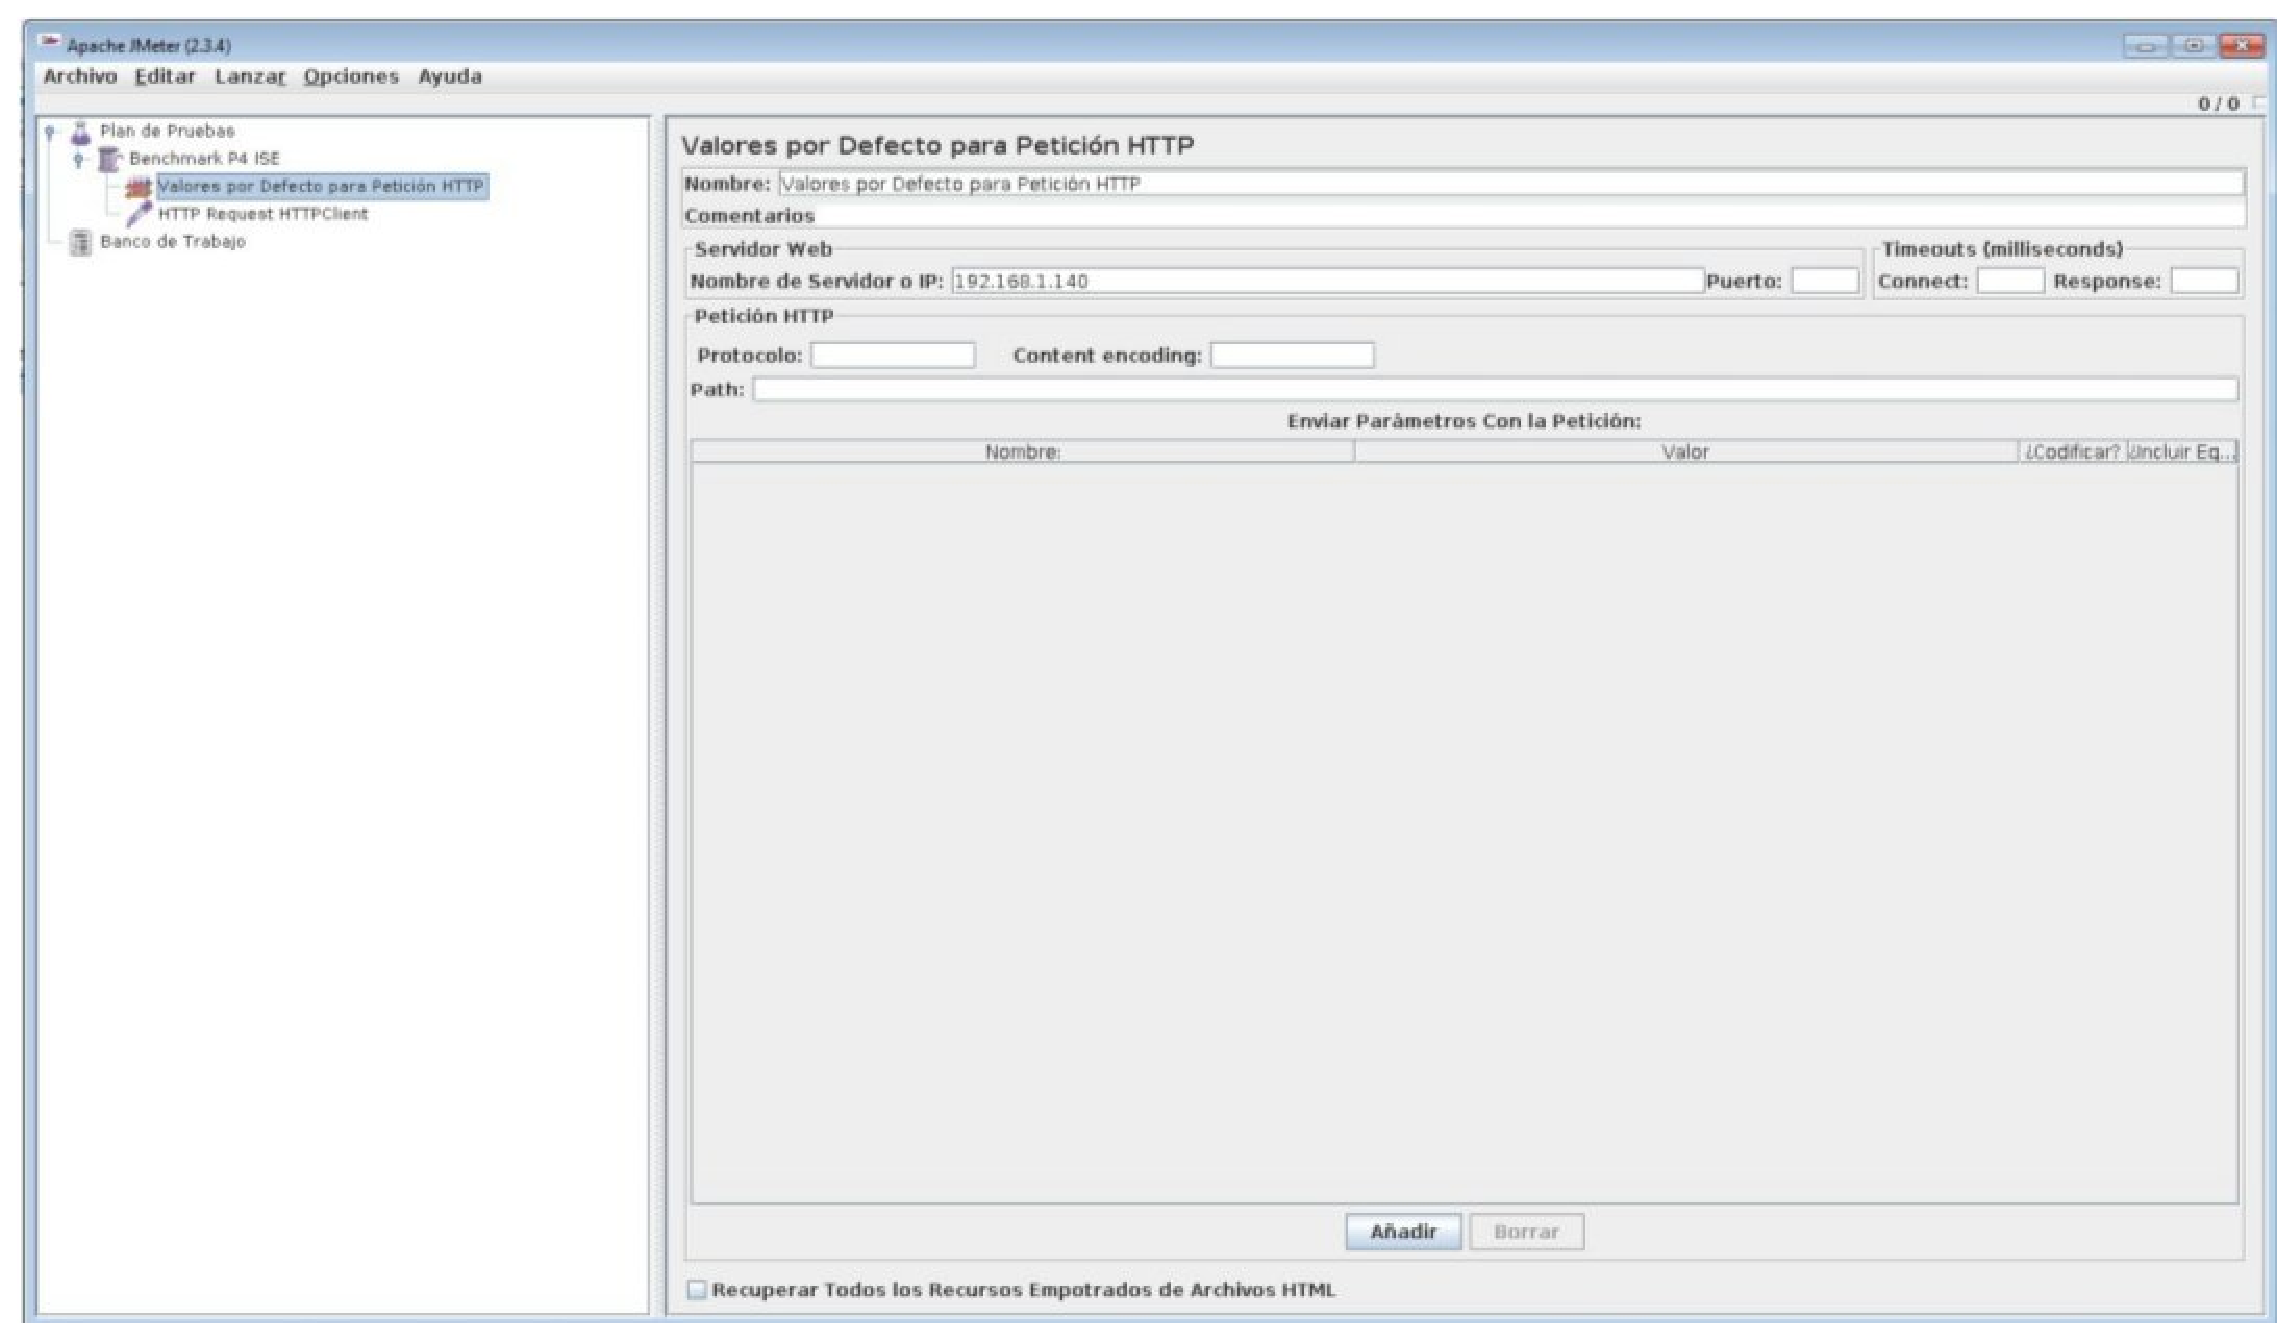
\includegraphics[scale=0.3]{imagenes/imagen4-3.eps}
\caption{Creacion de consultas HTTP.}
\end{center}
\end{figure}

\begin{figure}[H]
\begin{center}
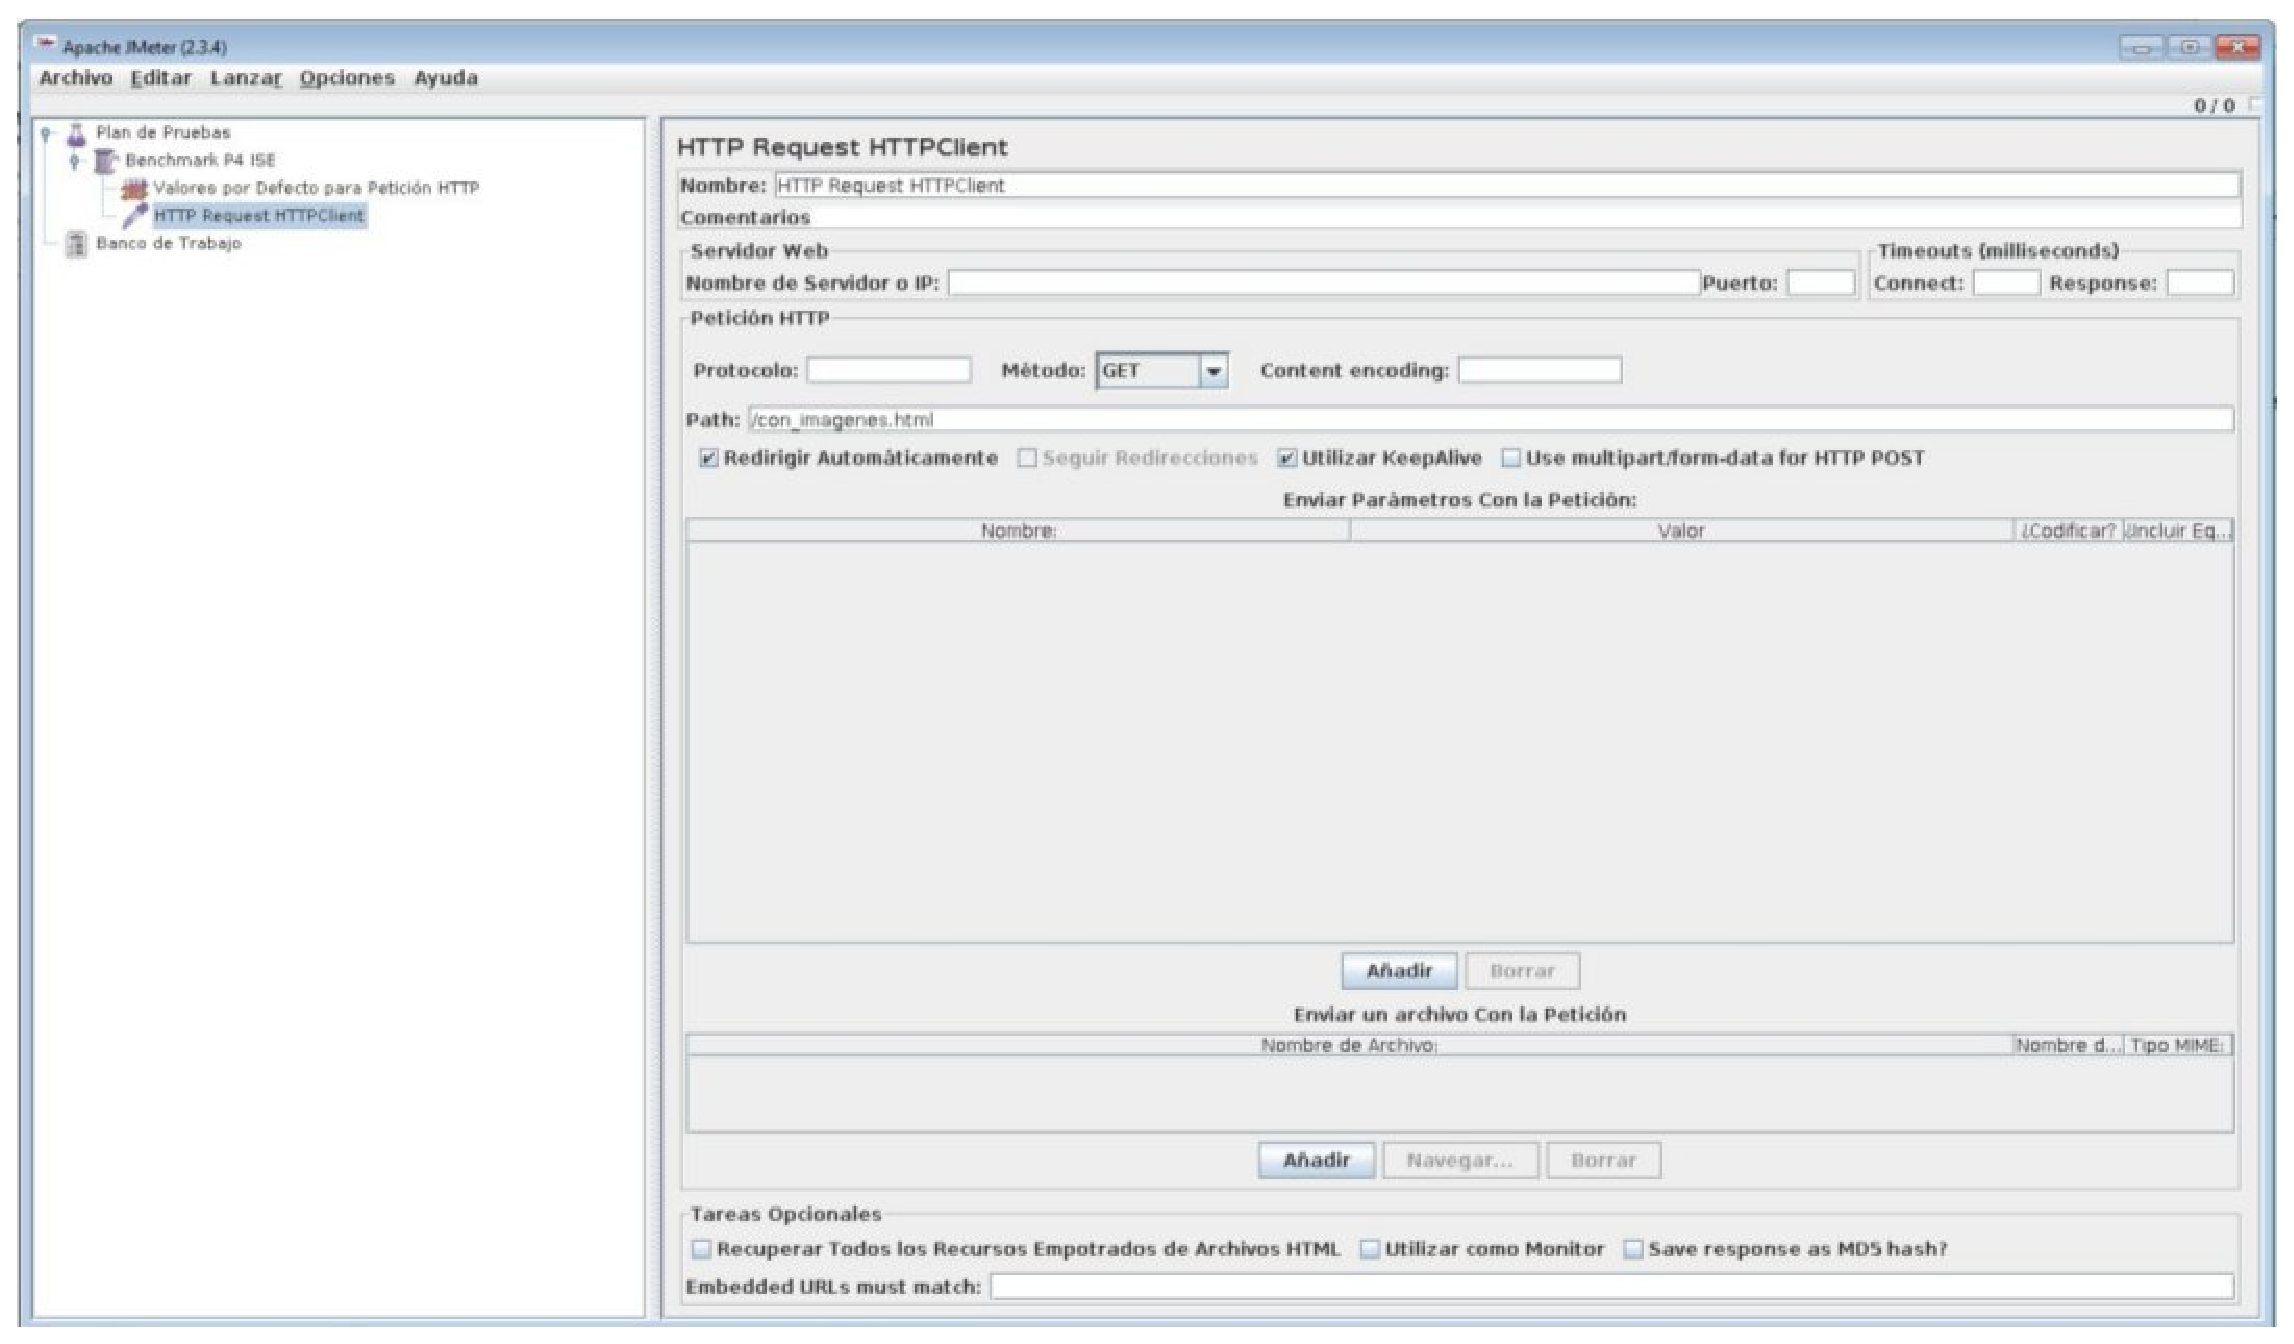
\includegraphics[scale=0.3]{imagenes/imagen4-4.eps}
\caption{creacion Request HTTPClient.}
\end{center}
\end{figure}
Por último, solo nos queda añadir el gráfico. Añadir -- Listener -- Gráfico de Resultados. Una vez creado, lo guardamos en donde queramos.
\begin{figure}[H]
\begin{center}
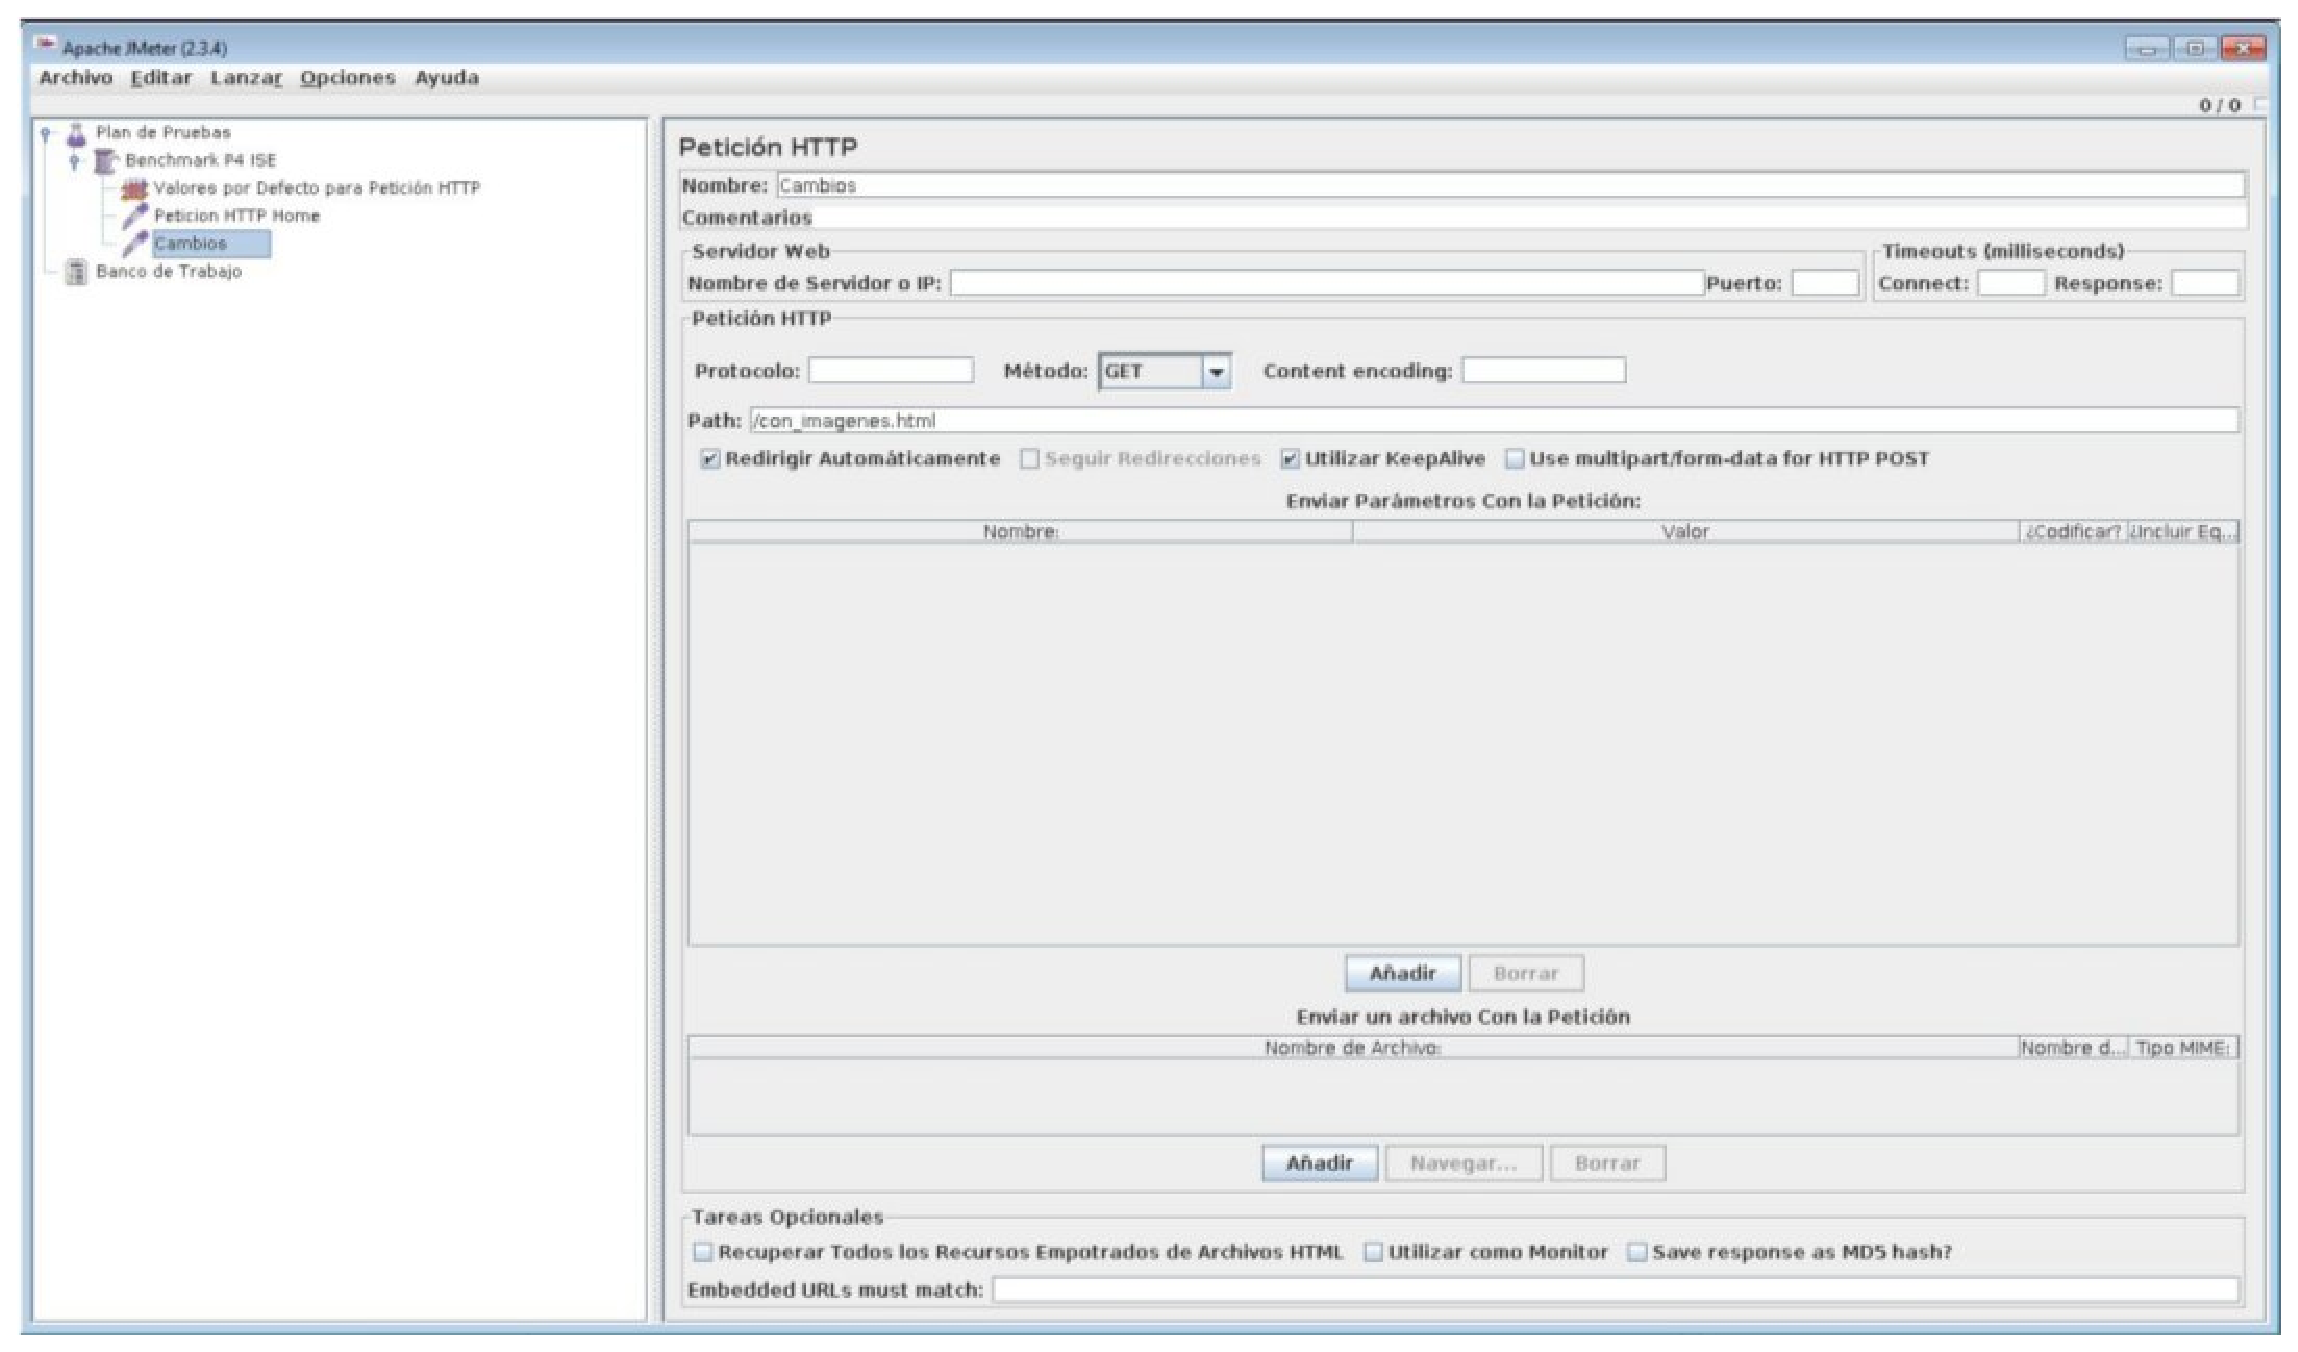
\includegraphics[scale=0.3]{imagenes/imagen4-5.eps}
\caption{Añadir el grafico de resultados.}
\end{center}
\end{figure}
Por último, ejecutamos (Lanzar -- Arrancar) y se generará un gráfico con los resultados:
\begin{figure}[H]
\begin{center}
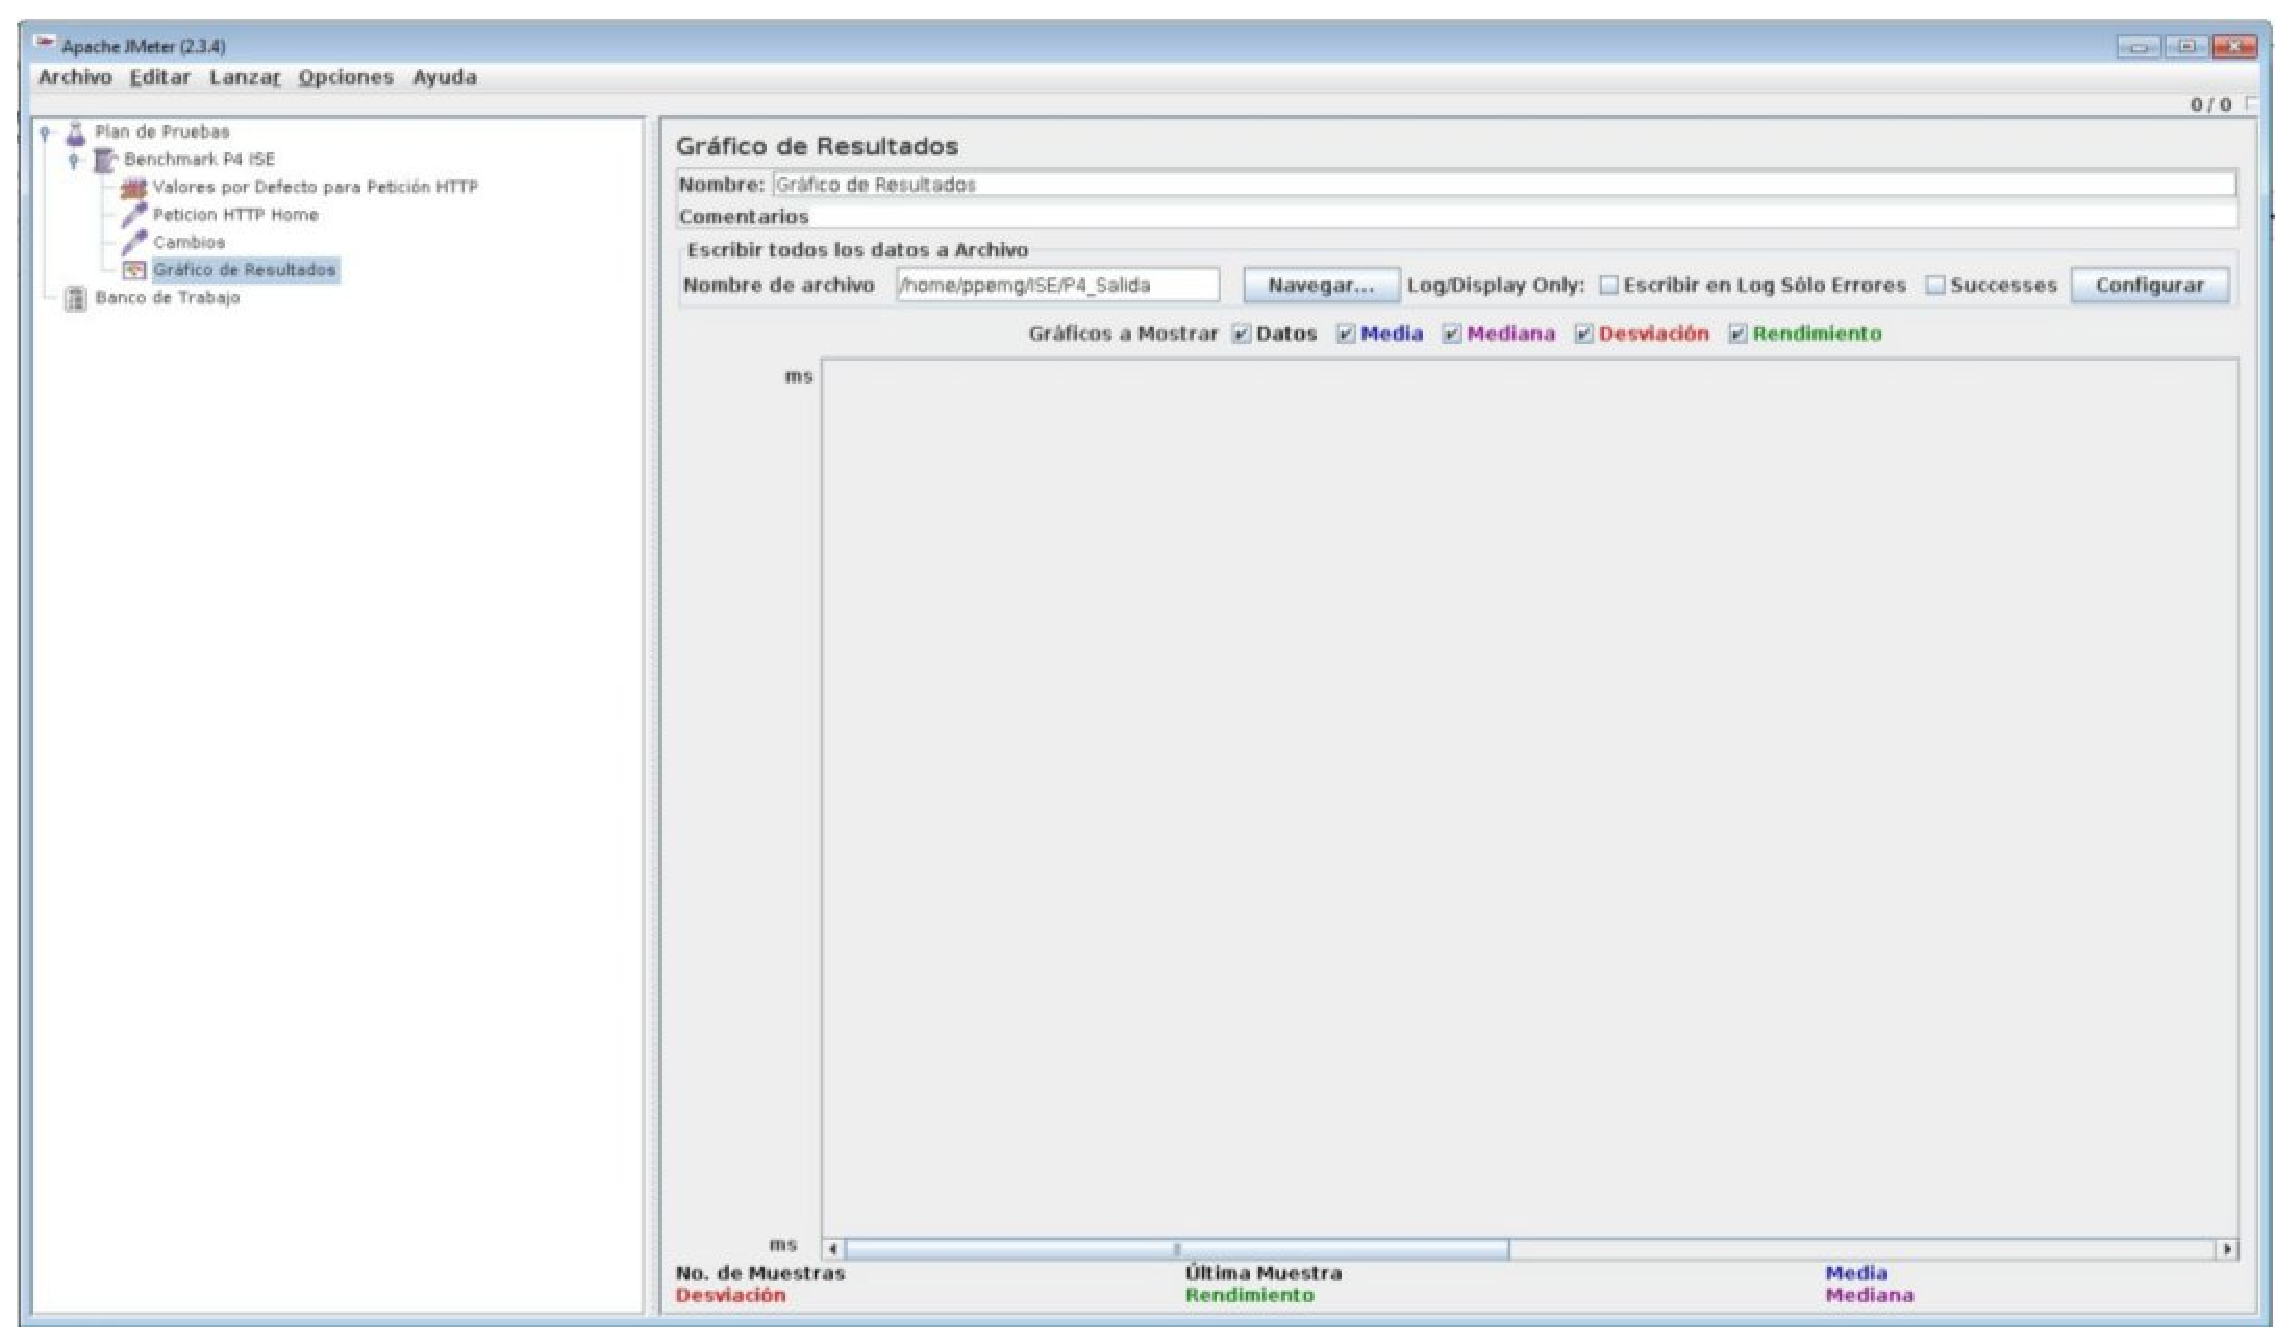
\includegraphics[scale=0.4]{imagenes/imagen4-6.eps}
\caption{Generación del gráfico.}
\end{center}
\end{figure}


\section{Programe un benchmark usando el lenguaje que desee. Elbenchmark debe incluir: 1) Objetivo del benchmark 2) Métricas (unidades, variables, puntuaciones, etc.) 3) Instrucciones para su uso 4) Ejemplo de uso analizando los resultados}
He hecho un benchmark para un test de CPU y de memoria.
He hecho un bucle que haga operaciones de suma, resta,division y multiplicacion. 
Respecto a la CPU he incluido unos calculos para punto flotante. Ademas, he intentado considerar el caso para multicpu con openmp.
Para el test de memoria tenia pensado realizar una ordenación por el algoritmo de la burbuja (por ejemplo) pero en lugar de eso he creado un vector de memoria dinamica e 2.500.000 enteros que son alrededor de 8.000.000 de bytes. Lo suficiente para que no quepa en la cahe. Accedo aleatoriamente a las posiciones del vector.
\begin{lstlisting}
/*
 * Benchmark para la asignatura de ISE.
 * Test de CPU y de Memoria.
 * 
 */
#include <iostream>
#include <fstream>
#include <ctime>

using namespace std;

int main(){
    
   clock_t tantes,tdespues;
   double tiempo;
   int puntuacion_cpu, puntuacion_mem;

   cout<<'\n';
   for(int i=0;i<30;i++) cout<<"*";
   cout<<"\n** BENCHMARK 0.1  **\n";
   for(int i=0;i<30;i++) cout<<"*";
   cout<<endl;

   //TEST DE CPU
   
   cout<<"\n### TEST DE CPU ### \n";

   int cantidad=0;
   double cantidad2=1.5;
   
   tantes = clock();
   
   cout<<"\nPasando test de CPU..."<<endl;
   #pragma omp parallel for
   for(int i=0;i<50000000;i++){
      cantidad = cantidad*2;
      cantidad = cantidad/2;
      cantidad++;
      cantidad--;
   }
   for(int i=0;i<5000000;i++)
      cantidad2=cantidad2*1.5;
   for(int i=0;i<5000000;i++)
      cantidad2=cantidad2/1.5;
   #pragma omp end parallel for

   tdespues = clock();
   
   tiempo = static_cast<double>(tdespues - tantes)/CLOCKS_PER_SEC;
   cout<<"\nTiempo empleado: "<<tiempo<<" segundos"<<endl;
   
   puntuacion_cpu = static_cast<int>(10000/tiempo);
   cout<<"\nPuntuacion obtenida: "<<puntuacion_cpu<<" puntos\n"<<endl;
   
  //TEST DE MEMORIA

	cout<<"\n\n### TEST DE MEMORIA ### \n";

	int *vector;
	int aux;
	vector = new int[2500000]; 

	tantes = clock();

	cout<<"\nPasando test de Memoria..."<<endl;
   #pragma omp parallel for
   for(int i=0;i<200;i++){
      //Escritura en vector
      for(int j=0;j<500000;j++)
         for(int k=0;k<2500000;k+=500000)
            vector[k+j]=j;
      //Lectura del vector
      for(int j=0;j<500000;j++)
         for(int k=0;k<2500000;k+=500000)
           aux = vector[j];
   }
   #pragma omp end parallel for

	tdespues = clock();
   
    tiempo = static_cast<double>(tdespues - tantes)/CLOCKS_PER_SEC;
	cout<<"\nTiempo empleado: "<<tiempo<<" segundos"<<endl;

    puntuacion_mem = 10000/tiempo;
	cout<<"\nPuntuacion obtenida: "<<puntuacion_mem<<" puntos\n"<<endl;
}
\end{lstlisting}
Para obtener una valoración he dividido 10000 entre el tiempo que tarda en ejecutarse, lo que me genera una puntuación. Con lo que a menor tiempo mayor puntuación.
Los resultados obtenidos son los siguiente:
\begin{figure}[H]
\begin{center}
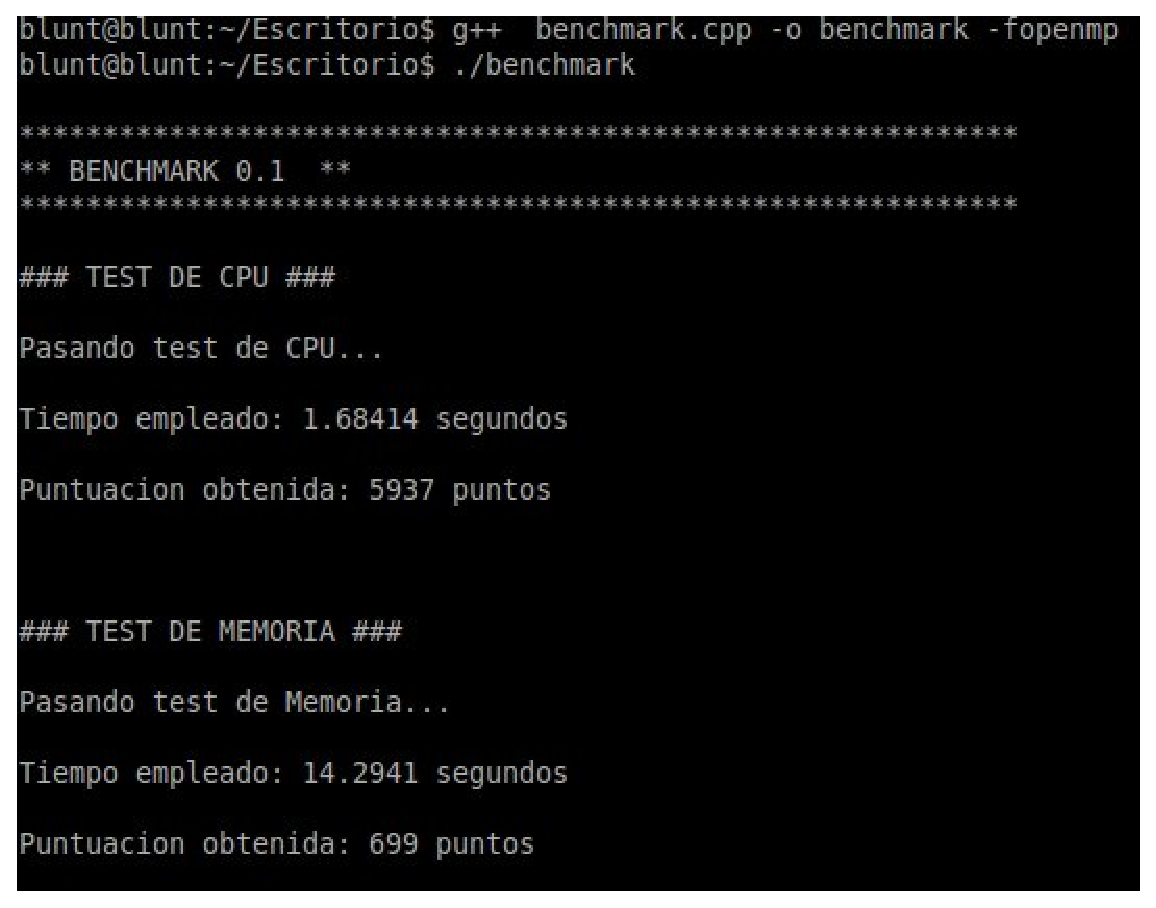
\includegraphics[scale=0.4]{imagenes/imagen5.eps}
\caption{Resultado de mi benchmark.}
\end{center}
\end{figure}
En la imagen se muestra que el tiempo de ejecución del test de CPU es menor y por tanto se obtiene una mayor puntuación.

\section*{Cuestion opcional 1. Seleccione, instale y ejecute uno, comente los resultados. Atención: no es lo mismo un benchmark que una suite, instale un benchmark.}
Para mas infomación sobre estos benchmark aconsejo la siguiente dirección \footnote{http://openbenchmarking.org/tests/pts}
.

Una podría ser el de "blogbench": 
- phoronix-test-suite install blogbench 
En \footnote{http://openbenchmarking.org/test/pts/blogbench} viene una descripción del funcionamiento del benchmark blogbench, cuya traducción literal es la siguiente.

Blogbench es un punto de referencia del sistema de ficheros portátil que intenta reproducir la carga de un servidor de archivos ocupado del mundo real. Hace hincapié en el sistema de archivos con múltiples hilos de realizar lecturas al azar, escribe y reescribe con el fin de tener una idea realista de la escalabilidad y la concurrencia de un sistema puede manejar.
En mi sistema una ejecución de este programa es la siguiente :

\begin{figure}[H]
\begin{center}
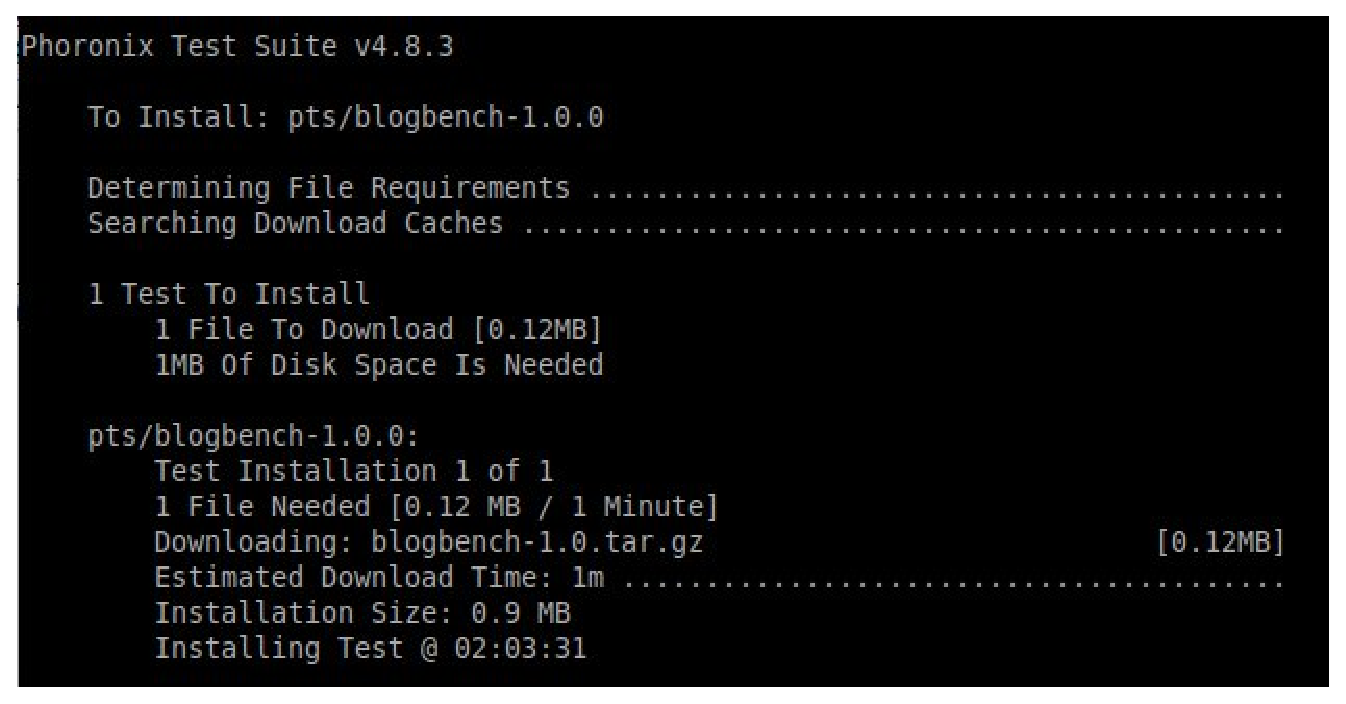
\includegraphics[scale=0.4]{imagenes/opcional1-1.eps}
\caption{Ejecucion de blogbench.}
\end{center}
\end{figure}



Y el último que vamos a probar es otro para procesadores llamado 
"bork", que al igual que el anterior \footnote{http://openbenchmarking.org/test/pts/bork} en su página tiene una definición de la labor que desempeña este benchmark : Bork es un pequeño, multiplataforma herramienta de cifrado de archivos. Está escrito en Java y diseñado para ser incluido junto con los archivos que cifra para el almacenamiento a largo plazo. Esta prueba mide la cantidad de tiempo que se necesita para cifrar un archivo de ejemplo.
Para ejecutarlo introducir el siguiente comando.
- phoronix-test-suite benchmark bork 
\begin{figure}[H]
\begin{center}
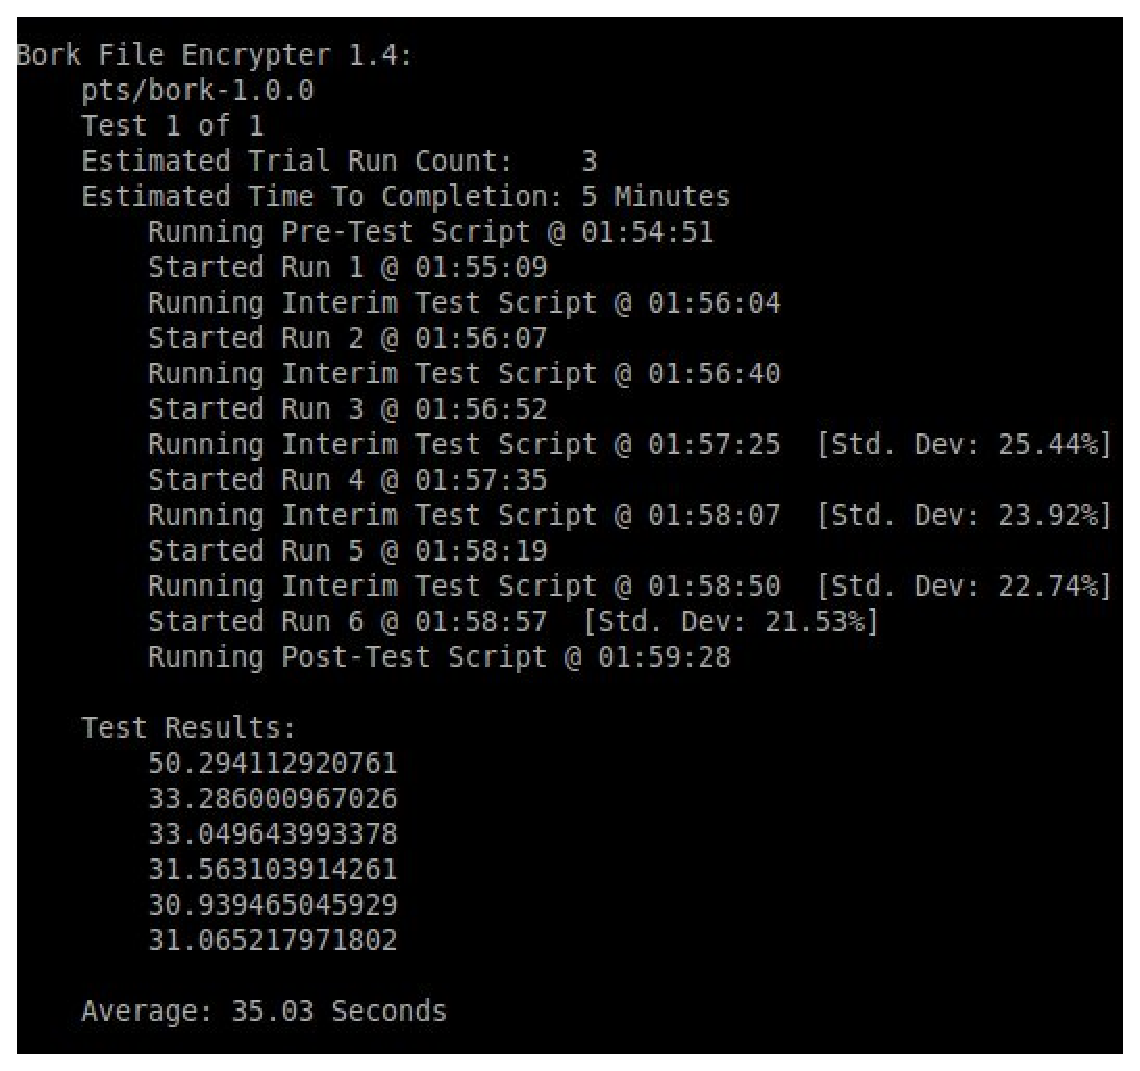
\includegraphics[scale=0.4]{imagenes/opcional1-2.eps}
\caption{Ejecución del bork.}
\end{center}
\end{figure}


\section*{Cuestión opcional 2: ¿Qué es Scala? Instale Gatling y pruebe los escenarios por defecto.}

En primer lugar “Scala” es un lenguaje de programacion de proposito general diseñado par aexpresar patrones comunes de programacion de foroma concisa y elegante. Se integran las caracterisiticas d ellos elnguajes orientados a obejetos y funcional. Scala no es una extencion de Jaca pero es toatamelete interoperable con él.
Scala se traduce a bytecodes Java y la eficiencia de lso programas compilados por lo general es igual que Java.
Bueno pasando un poco de la teoría, vamos a instalarlo cn Ubuntu con el siguiente comando:
\textit{“sudo apt-get install scala”}

\begin{figure}[H]
\begin{center}
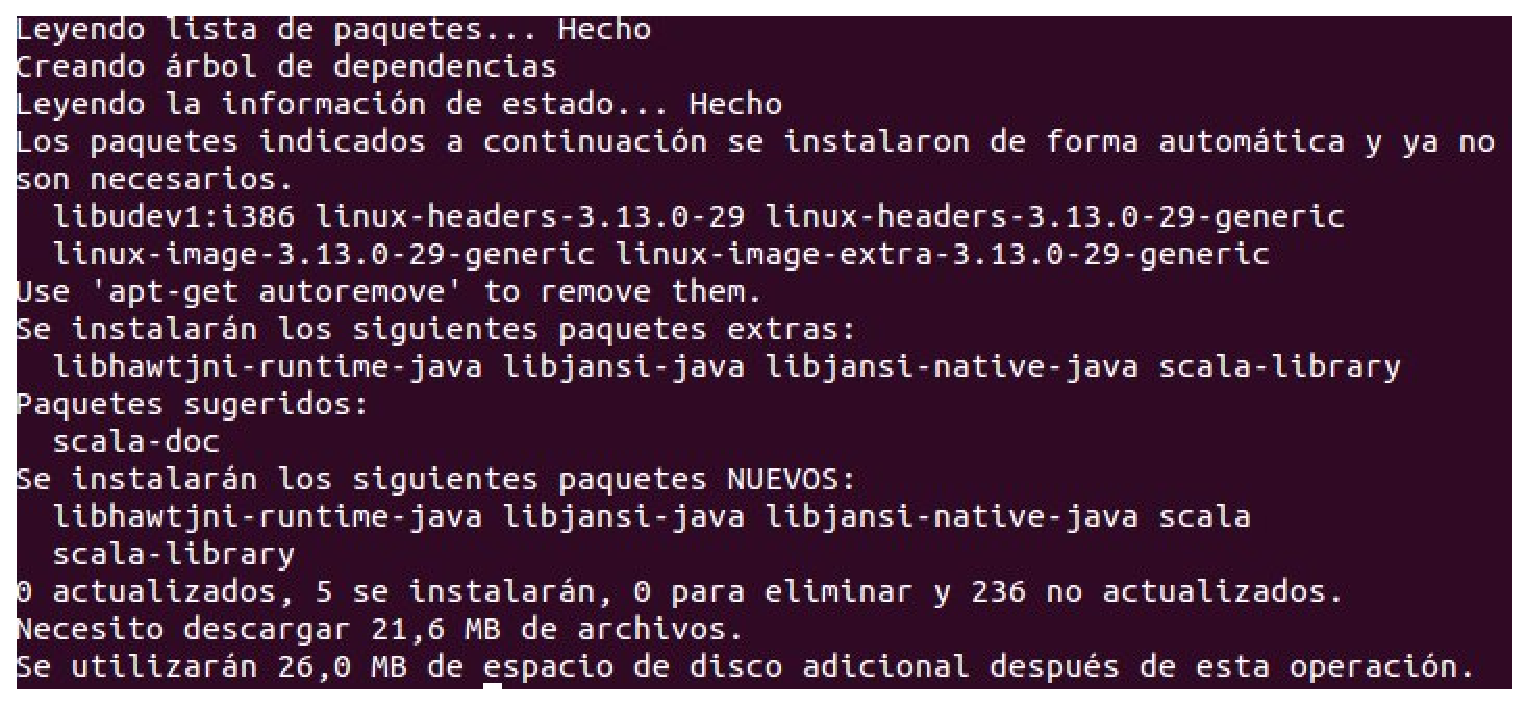
\includegraphics[scale=0.4]{imagenes/opcional2-1.eps}
\caption{Instalación de Scala.}
\end{center}
\end{figure}

El código de hola mundo seria el siguiente:\\
\begin{figure}[H]
\begin{center}
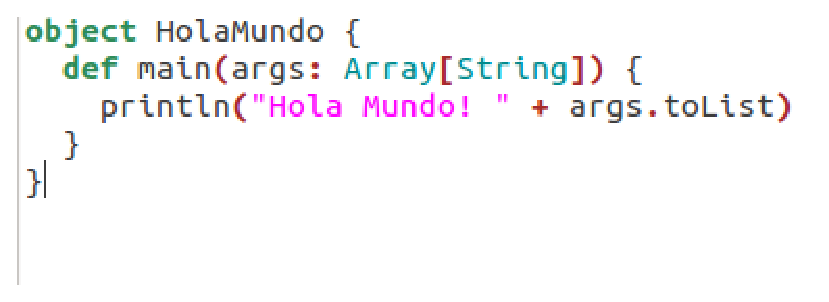
\includegraphics[scale=0.4]{imagenes/opcional2-2.eps}
\caption{Código de hola mundo.}
\end{center}
\end{figure}

Guardaremos el codigo anterior para poder compiilarlo con el siguiete comando.

\begin{figure}[H]
\begin{center}

\includegraphics[scale=0.4]{imagenes/opcional2-3.eps}
\caption{Ejecución programa en Scala.}
\end{center}
\end{figure}


Una vez compilado obtendremos dos nuevos archivos holaMundo.class u holaMundo \$.class.
Si hay errores durante la  compilacion seran mostrados en el terminal.
\begin{figure}[H]
\begin{center}
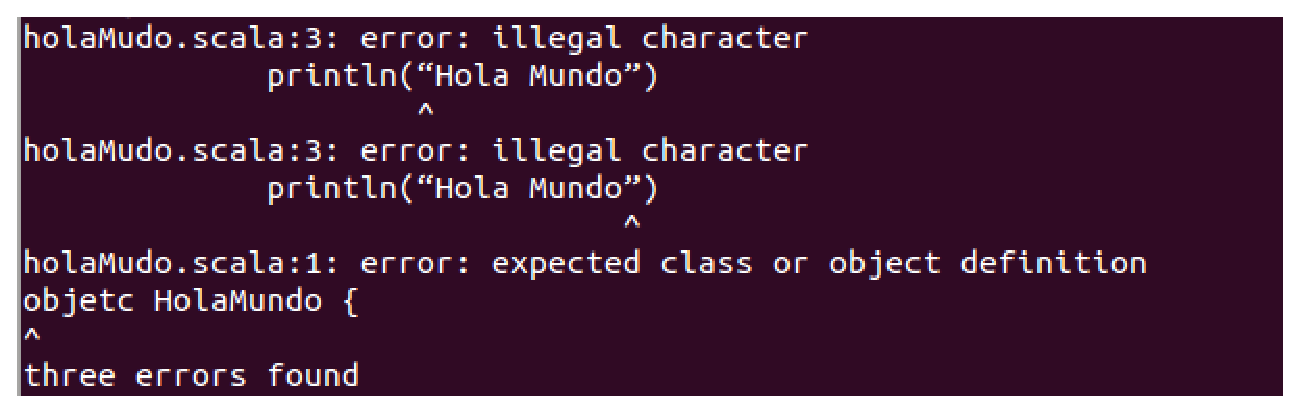
\includegraphics[scale=0.4]{imagenes/opcional2-4.eps}
\caption{Errores en Scala.}
\end{center}
\end{figure}

El terminal nos muestra la salida del programa. List() nos indica los parametros que le pasamos a la funcion. Esto se muestran por pantalla por la linea:

\textit{println("Hola Mundo! " + args.toList);}

El resultado es el siguiente:

\textbf{Hola Mundo! List(Parametro1, Parametro2)}
\begin{figure}[H]
\begin{center}
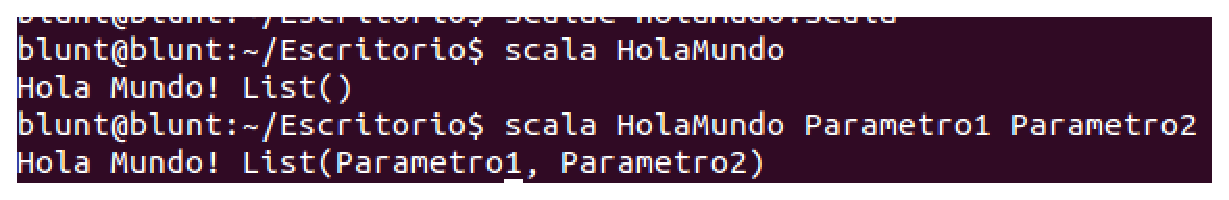
\includegraphics[scale=0.4]{imagenes/opcional2-5.eps}
\caption{Ejecución programa con Scala.}
\end{center}
\end{figure}

Para instalar Gatling en Ubuntu podemos hacerlo desde los repositorios que vienen incluidos con el siguiente comando \textit{sudo apt-get install gatling}.
\footnote{http://gatling.io/docs/1.5.6/user\_documentation/tutorial/first\_steps\_with\_gatling.html\#first-steps-with-gatling}
\section*{Cuestión opcional 3: Lea el artículo y elabore un breve resumen.}
El articulo hace una comparación entre dos benchmark conocidos; Gantling y Jmeter.

El articulo muestra su total apoyo a ambos proyectos y realiza comparaciones de los benchmark en distintas situaciones mostrandos sus diferencias en unas graficas de memoria y CPU, al final muestran sus diferencias y las conclusiones  a las que llegan:
\\
\\
\textit{"Tanto JMeter y Gatling demostraron las características deseadas de relativamente planas tiempos de respuesta de las transacciones medidas durante RampUp y bajo carga, con poca variación. Tiempo medio de respuesta no debe ser utilizado como una medida del rendimiento de la herramienta a un lado de la observación previa en este sentido. Tanto JMeter y Gatling fueron capaces de mantener un rendimiento promedio en la región de 30.000 peticiones por minuto con ninguna desviación. Tanto JMeter y Gatling fueron RampUp capaz de 10.000 usuarios simultáneos en 10 minutos, que se considera normalmente un objetivo agresivo desde un solo generador de carga. Tanto JMeter y Gatling demostraron comportamiento de caché correcta, sobre todo cuando hace peticiones condicionales para recursos estáticos que responden con un HTTP 304. Gatling fueron capaces de proporcionar rápidamente con un parche para asegurar que este . Ambos planes de prueba JMeter y Gatling incluyen extracción de contenido a través de expresiones regulares desde el cuerpo de la respuesta, así como las afirmaciones de texto y códigos de respuesta HTTP contenidos sin menoscabo de su rendimiento."}
\\
En definitiva el articulo no recomienda uno u otro, termina diciendo que el uso de uno u otro en mas bien " subjetivo".
\section*{Cuestión opcional 4: Seleccione un benchmark entre SisoftSandra y Aida. Ejecútelo y muestre capturas de pantalla comentando los resultados.}
\footnote{http://www.sisoftware.co.uk/}
He elegido SisoftSandra.
\\
He realizado dos tests, con dos configuraciones distintas: 
\\
1a 4 CPU – 1 GB de RAM 
\\
2a 2 CPU – 2 GB de RAM 
\\
Realizamos los dos test, y obtenemos dos gráficos:
\begin{figure}[H]
\begin{center}
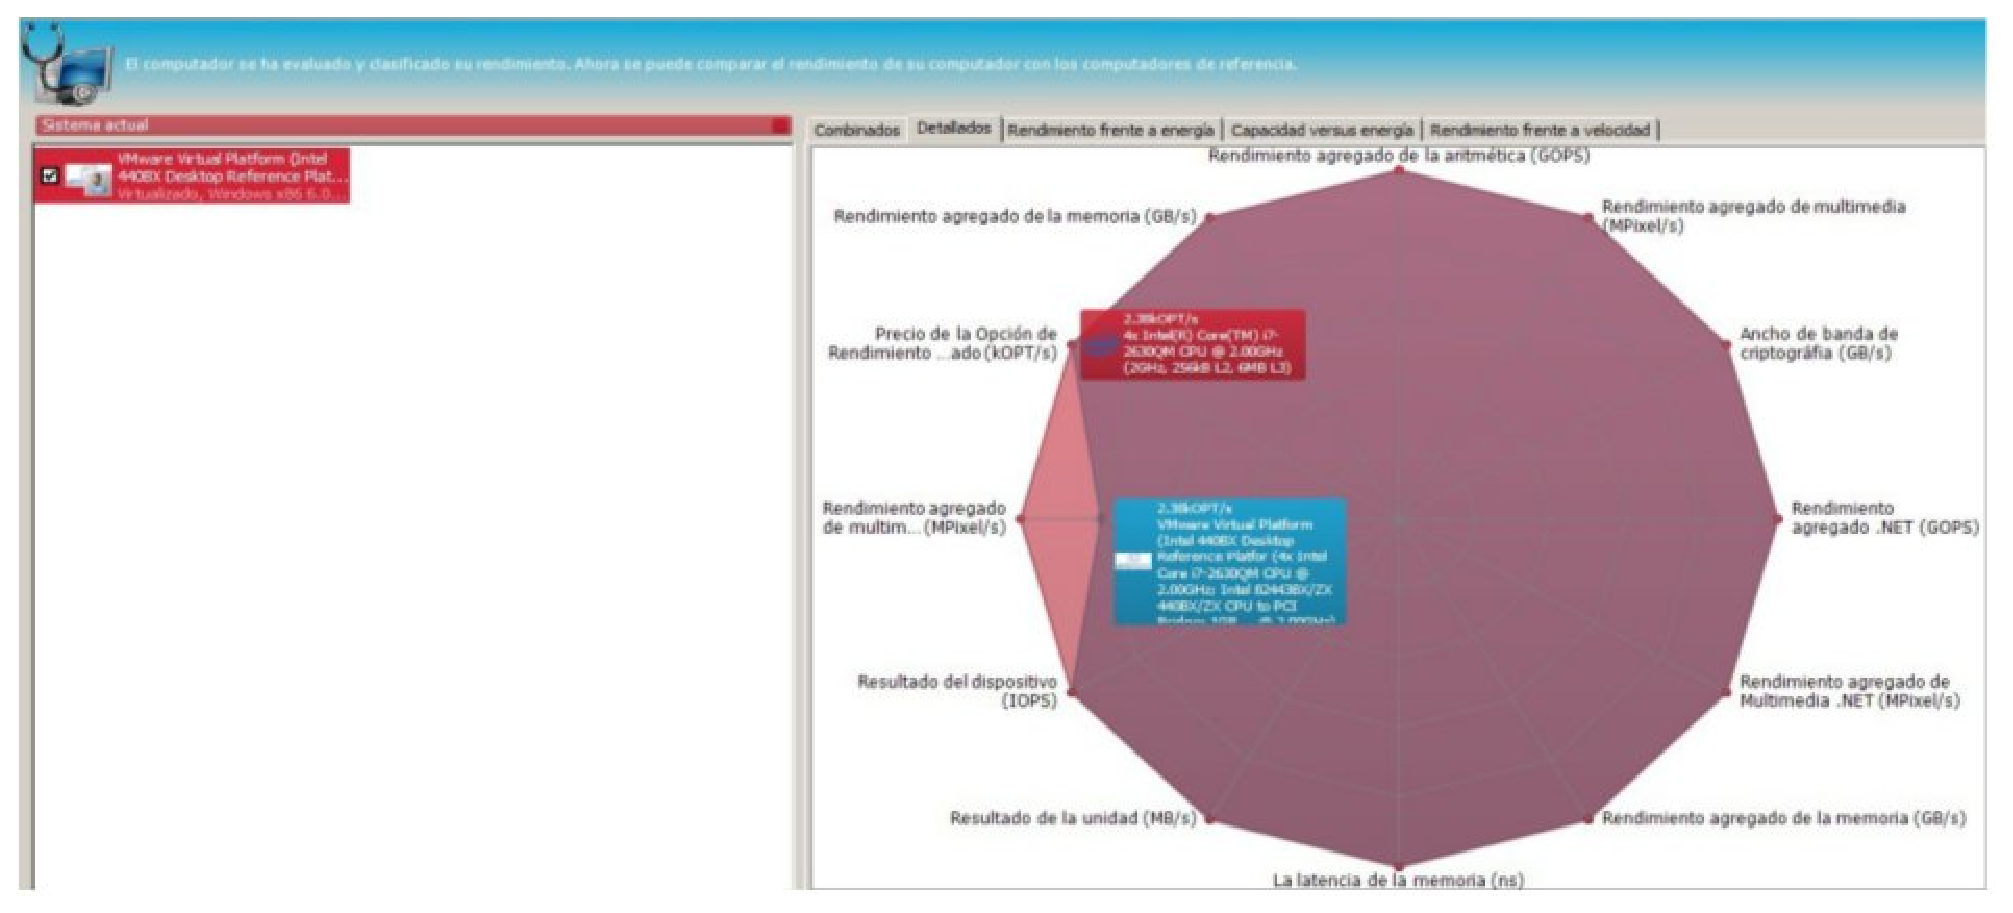
\includegraphics[scale=0.4]{imagenes/opcional4-1.eps}
\caption{Grafico de la primera configuración.}
\end{center}
\end{figure}
Después, cambiamos las opciones de la máquina virtual para establecer la segunda configuración y volvemos a pasar el benchmark. Hecho esto, obtenemos:
\begin{figure}[H]
\begin{center}
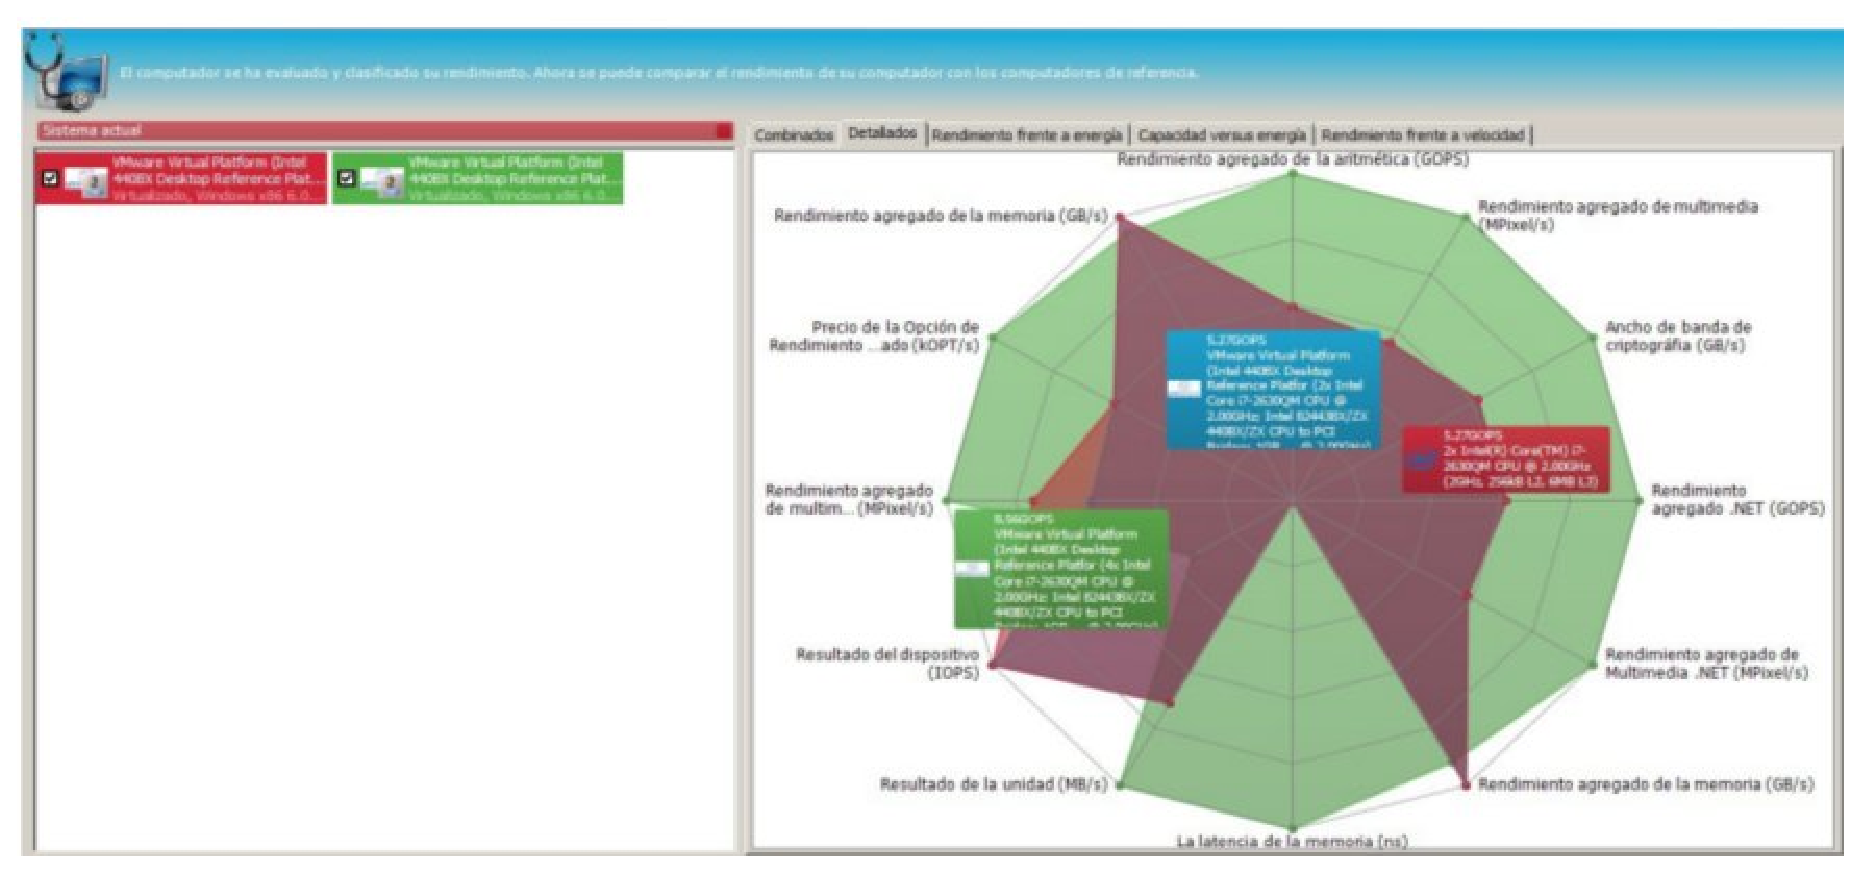
\includegraphics[scale=0.4]{imagenes/opcional4-2.eps}
\caption{Segunda configuración.}
\end{center}
\end{figure}

Cómo vemos, la configuración de dos procesadores es inferior a la de 4 en 
rendimiento del procesador (lógicamente) pero hay algunas áreas en las que se nota 
el aumento en la memoria RAM. 
\end{document}